\documentclass[a4paper, 11pt, oneside, polutonikogreek, german]{article}
\usepackage{ebgaramond}
% Load encoding definitions (after font package)
\usepackage[LGR,T1]{fontenc}
\usepackage{textalpha}
\usepackage{graphicx}
\usepackage{float}
\graphicspath{ {./} }
\usepackage[figurename=]{caption}
\usepackage{listings}
\usepackage{subcaption}
\lstset{basicstyle=\ttfamily}

% Babel package:
\usepackage{babel}
% With XeTeX/LuaTeX, load fontspec after babel to use Unicode
% fonts for Latin script and LGR for Greek:
\ifdefined\luatexversion \usepackage{fontspec}\fi
\ifdefined\XeTeXrevision \usepackage{fontspec}\fi

% "`Lipsiakos" italic font `cbleipzig`:
\newcommand*{\lishape}{\fontencoding{LGR}\fontfamily{cmr}%
		       \fontshape{li}\selectfont}
\DeclareTextFontCommand{\textli}{\lishape}

\usepackage{booktabs}
\setlength{\emergencystretch}{15pt}
\usepackage{fancyhdr}
\usepackage{microtype}
\begin{document}
\begin{titlepage} % Suppresses headers and footers on the title page
	\centering % Centre everything on the title page
	%\scshape % Use small caps for all text on the title page

	%------------------------------------------------
	%	Title
	%------------------------------------------------
	
	\rule{\textwidth}{1.6pt}\vspace*{-\baselineskip}\vspace*{2pt} % Thick horizontal rule
	\rule{\textwidth}{0.4pt} % Thin horizontal rule
	
	{\scshape\LARGE Die Göttin von Paphos \\ auf alten Bildwerken \\ und Baphomet}
	
	\rule{\textwidth}{0.4pt}\vspace*{-\baselineskip}\vspace{3.2pt} % Thin horizontal rule
	\rule{\textwidth}{1.6pt} % Thick horizontal rule

	%------------------------------------------------
	%	Subtitle
	%------------------------------------------------

        \vspace{1\baselineskip}
    
	{\scshape Von \Large C. G. Lenz} % Subtitle or further description

        \vspace*{\fill}
    
        {\scshape\small --- Argentum et marmor vetus aeraque et artes suspice. \\\hspace*{33mm}Horat.} % Subtitle or further description
    
    %------------------------------------------------
	%	Cover photo
	%------------------------------------------------
	
	
	%------------------------------------------------
	%	Editor(s)
	%------------------------------------------------
        \vspace*{\fill}

	\vspace{1\baselineskip}

	{\small\scshape Gotha, 1808}
	
        \vspace{0.25\baselineskip}
 
        {\scshape\footnotesize Mit Reiherschen Schriften}
        
	\vspace{0.5\baselineskip} % Whitespace after the title block

        {\small\scshape Solar Anamnesis Edition} % Publication year
	
	{\scshape\small CC0 1.0 Universell} % Publisher
\end{titlepage}
\setlength{\parskip}{1mm plus1mm minus1mm}
\clearpage
\begin{figure}[H]
\centering
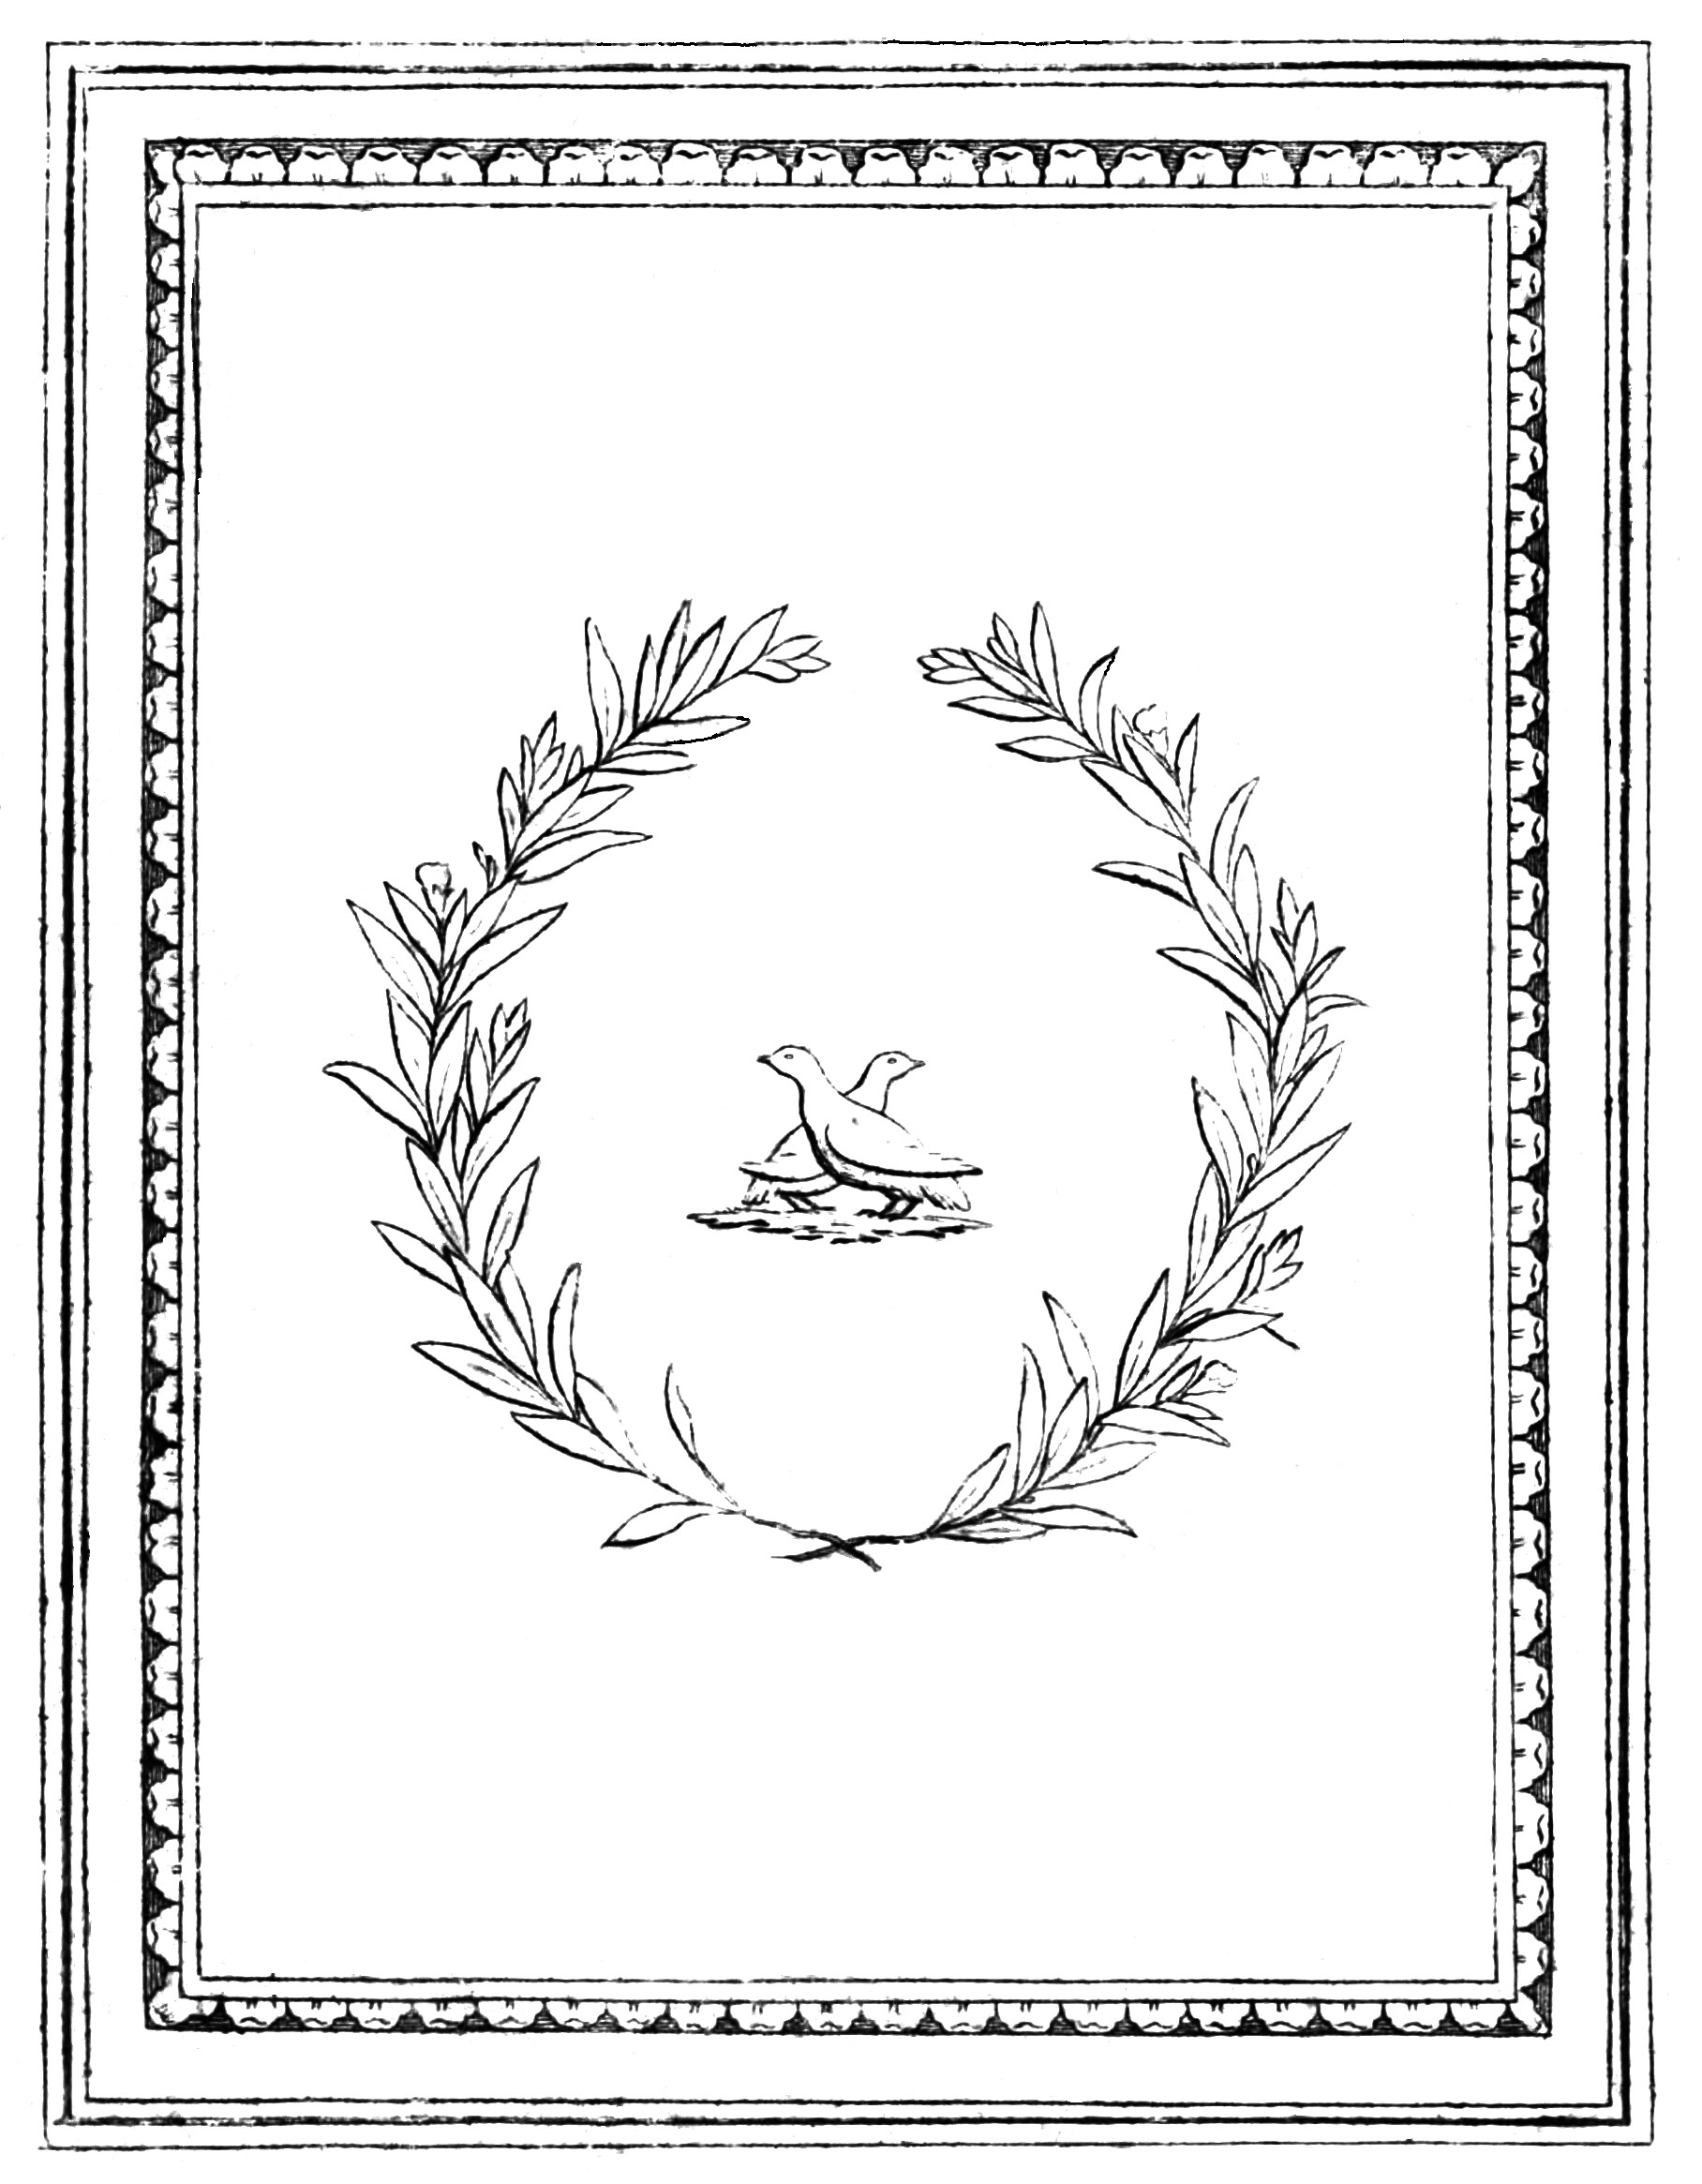
\includegraphics[width=0.95\textwidth,keepaspectratio]{fig1.jpg}
\end{figure}
\clearpage
\paragraph{}
Die in Asien weit umher verbreitete Anbetung der Himmels-Königin\footnote{Über die große Natur-Göttin, welche vielfältig an Namen, aber Eine dem Begriff nach war, haben nach Seldenus unsre neuern Mythologen, Heyne, Böttiger, Heinrich, Creuzer, Wagner u. a. m. lichtvollere Ansichten verbreitet. Vorzüglich gebührt hier eine ehrende Meldung der reichhaltigen Heynischen Vorlesung de sacerdotio Comanensi omninoque de religionum cis et trans Taurum consensione, welche unlängst im 16\textsuperscript{ten} Bande der Commentatt. soc. reg. Gotting. erschienen ist.} wird in diesen Blättern nur insofern berührt werden, als sie in die Erläuterung der alten Denkmäler, die das Bild der Paphischen Göttin und ihren Tempel darstellen, einfließt. Je dürftiger die Nachrichten der Schriftsteller über das Tempel-Gebäude der Paphia, desto beredter sind die Abbildungen, und die Münzen insonderheit geben eine Folge von Darstellungen, die als eine fortlaufende Geschichte des Tempels und seiner Schicksale angesehen werden mögen. Denn anstatt dass die Steinschneider die Fabel und Geschichte mehr als freies Spiel der Phantasie behandelten, banden sich die Verfertiger von Münz-Stämpeln an die Wahrheit der Geschichte, deren Tatsachen sie in dauernden Urkunden der Nachwelt treuer überlieferten. Ihnen dürfen wir daher als zuverlässigen Führern folgen, wenn sie uns National-Denkmäler abbilden, obgleich eingedenk, dass sie beschränkt durch die Gränzen der Kunst und die Enge des Raums oft nur unvollständige Nachbildungen geben können, dass sie unwesentliche Teile weglassen und in Neben-Dingen bald mit Vorbedacht bald aus Unachtsamkeit vom Urbild abweichen.\footnote{Heyne hat in den Gött. gel. Anz. 1807 St. 203 eine Untersuchung hierüber eingeleitet, welche Levezow in der Schrift über die Mediceische und die Knidische Venus Berl. 1808 durch besondere Erörterung der Frage: Inwiefern sind auf den Münzen des Altertums gültige Abbildungen ehemals berühmter und ausgezeichneter Kunstwerke enthalten S. 46 ff. weiter ausgeführt hat.}

Uralt war Tempel und Bild der himmlischen Aphrodite auf Paphos in Kypern; Muster-Tempel desselben war der der Urania zu Askalon (Herodot. 1., 105): mit Kypros befreundete Städte, als Pergamos und Sardes, erkannten ebenfalls die Paphische Göttin an, wie ihre Münzen ausweisen, und auch in Thalamae im Lakedämonischen Gebiet war ihr Bild in dem unbedeckten Teile des Tempels (Pausan. 3, 26) neben dem Helios aufgestellt.

Von ihrem Tempel-Gebäude nachher besonders; itzt von der sonderbaren Gestaltung der Göttin. Ein Blick auf die Münzen und andern Abbildungen des Altertums, welche auf zwei Blätter dieser Schrift zusammengedrängt worden,\footnote{Ich habe mich dabei des Steindrucks, der zu Umrissen dieser Art so sehr geeignet ist, bedient, da mir der Herr Hauptmann v. Schlotheim in Gotha, der sein Talent und seinen Kunstfleiß auf die Ausübung dieser schätzbaren Erfindung zu verwenden anfängt, in Gemeinschaft mit dem jüngeren Hn. Döll, der die Zeichnungen unter meinen Augen besorgt hat, dazu die Hand bot. Die meisten Münzen waren mir im herzogl. Gotischen Münz-Kabinett teils selbst teils in Mionnets Schwefel-Abdrücken vor Augen, und nur bei wenigen musste ich mich auf Abbildungen in Münzwerken verlassen.} zeigt sie als Kegel oder rundlichen Stein, ein Nachlass der alten kunstlosen Zeit, welche die Götter durch rohe, gestaltlose Stein-Klumpen darstellte.\footnote{Eine reiche Beispiel-Sammlung bietet Zoëga de obeliscis p. 194 ff. dar. Unter diesen kommen auch Sonnen- (Sol Elagabalus) und Mond-Steine (Urania, Mond) vor, die vom Himmel herabgefallen waren und die schon ihres Ursprungs halber auch in späterer Zeit ihre rohe Ungestalt behielten.} Aber an dem unbehauenen Stein, der ursprünglich der Paphia unwürdiger Stellvertreter gewesen sein mag, verrät sich auf unsern Denkmälern schon mehr oder weniger die bildende Hand des Menschen, die den Stein allmählig mehr abrundet, zuspitzt, etwas kopfähnliches ansetzt, Spuren von Händen hervorgehen lässt, und sonst vielleicht durch Umrisse, Einschnitte und Zeichen Natur und Geschlecht andeutet. Und so ließe sich überhaupt durch eine lange Induktion aus Münzen der stufenweise Übergang von den unorganisierten Massen zu gegliederten Götter-Wesen anschaulich machen.\footnote{Vgl. z. B. Pausan. 3, 19 und Heynes Bemerkungen über diese Stelle in den antiquar. Aufsätzen St. 1 S. 71 f.} Die Steine gestalten sich, wie nach Deukalions Flut, nach und nach menschlich.

Genauer die Gestalt der Paphia zu bestimmen, hören wir zuerst die Schriftsteller ab, deren Aussagen Meursius (Cypro 1, 16) gesammelt hat. Tacitus (Hist. 2, 3) sagt, dass sie nicht in Menschen-Gestalt vorgestellt sondern unten kreisförmig und breit sei (continuus orbis latiore initio), aber nach oben wie ein Kegel dünner werde (tenuem in ambitum metae modo exsurgens.) Maximus Tyrius (or. 38): sie lasse sich keiner andern Gestalt besser vergleichen als einer weißen Pyramide. Servius (Aen. 1) gibt ihr die Gestalt "`eines Nabels, oder, wie andere wollen, eines Kegels"' (in modum umbilici, vel, ut quidam volunt, metae colitur). Das Wesentliche bleibt also ein kegelartig gestalteter dicker, bauchiger oder nabelförmiger Stein, den aber Zeit und Kunst allmählig mehr auszierte und gliederte.\footnote{Curtius 4, 7, 23 gibt, wie die Alten der Paphierin, so dem Orakelgott Ammon in Libyen die Nabel-Gestalt: umbilico maxime similis est habitus: welches auch von einem rundlichen, Hermenartigen Stein zu verstehen sein wird, ähnlich dem Bildnis Ammons in Megalopolis in Arkadien, das Pausanias 8, 32, 1 mit den viereckten Hermen vergleicht, und von dem er sagt, dass es Widder-Hörner am Kopf habe. Oder dachte sich Curtius den Libyschen Gott in Gestalt eines Ammons-Horns? Es wäre doch so unnatürlich nicht, wenn ihm, dem Gott der verwickelten und künstlich gedrehten (λοξὰ) Orakel-Sprüche, die Phönizier, durch die er bekannt wurde, eine gedrehte und gewundene Konchylien-Form gegeben hätten, wie sie ihrer Astarte die Dionaea oder Venus-Muschel als Sinnbild beigelegt haben sollen (s. Böttiger N. T. Mercur 1805 St. 3 S. 219), worauf sich, wenn man anders nötig hätte so weit zu gehen, auch die Nabel-Gestalt der Paphia zurückführen ließ. Merkwürdig ist immer, was nur Joh. Lydus (de mensib. p. 9) berichtet, die Aphrodite sei bei den Phöniziern Blatta nach der Purpur-Schnecke genannt worden. Vgl. über das Wort blatta Tzschuckes gelehrte Ausführung zu Eutrop. 7, 14 p. 478 f. der großen Ausg. nebst dem Ind. notar. h. v. "`fert blattam Tyrus"' Sidon. Carmen 5, 48.}

Auf einigen unsrer Münzen und andern Bildwerken erscheint die Göttin völlig als Pyramide, auf andern mehr oder weniger abgerundet und kegelförmig, meistens mit einem Aufsatz von Knopf oder Calathus,\footnote{Am größten und auffallendsten erscheint dieser Aufsatz der Meta in 1., 13.} welches der Gestalt schon ein kopfähnliches Ansehen gibt, und endlich auf ein paar mit Extremitäten zu beiden Seiten, die wie Handhaben aussehen und sich als Vorbilder von Händen oder Armen betrachten lassen. Auch Spuren von Figuren oder Hieroglyphen lassen sich auf einigen entdecken. Der Nabel- und Kugel-Gestalt nähert sich am meisten die Münze des Vespasianus im herzogl. Gotischen Kabinett (1., 2), die, um ihren Charakter kurz auszudrücken, wie ein Kanobus-Bild aussieht.

Nun wurden in der Kanobus-Gestalt, die man den heiligen Nilkrügen in Ägypten gab, die großen Phönikischen Götter, welche unter den Namen Kabiri, Patäki, Dioskuri, begriffen wurden und mit denen auch späterhin Kastor und Pollux zusammenschmolzen, häufig dargestellt. Ihre Zahl ist unbestimmt; denn bald werden ihrer zwei, Himmel und Erde, bald drei, bald mehrere genannt; die große Natur-Göttin gehört ihnen an, teilt also auch ihre Gestalt.\footnote{Die neuesten und zwar erschöpfenden Untersuchungen über diesen Gegenstand sind in Creuzers Dionysus P. 1 angestellt. Völlig durchgeführt wird er erst im zweiten Teil werden; dort wird man auch bestimmt erfahren, wie sich der Vf. die Entstehung der Sage von Kanobus, dem Steuermann des Menelaus, erklärt. Es war vermutlich einer von Helenas Brüdern, welche nachmals, mit den alten Samothrakischen Dioskuren oder Kabiren verwechselt, auch als Kanoben vorgestellt wurden.}

Diese Klasse von Göttern nun wird gewöhnlich als ellenhohe oder noch kleinere Pygmäen geschildert, die man schon um ihres geringen Umfangs willen als Aufsätze mit sich herumtrug, als Haus-Götter und Schützer der Gastmahle auf die Tafeln setzte, und dann auch als Wasserkrüge, "`mit ganz kleinen Füssen, zusammengezogenem Halse und einem gleichsam aufgeschwollenen, dicken Bauche, der nach Art einer Hydria mit dem Rücken gleich rund ist"' (Rufin, Kirch. Gesch. 11, 26) vorzustellen liebte. Unter diesen tragbaren Göttern, die man auf die Tische stellte (Epitrapezii), wird vorzüglich Herakles genannt, der bei den Ägyptern und Phöniziern als Sol den Patäki oder Kabiri zugesellt wurde.\footnote{Siehe über diese kleinen Tischgötter, nach Seldenus, besonders Creuzer S. 136 ff.} So findet man beim Pausanias (8, 31) einen Herakles in Arkadien erwähnt, der vor einer kolossalen Bildfäule der Demeter stand und höchstens eine Elle hoch war. "`Dieser Herakles, fährt Pausanias fort, soll einer von den Idaei Daktyli gewesen sein, wie Onomakritos in seinen Gedichten sagt."' Und so wird auch einer sehr alten tragbaren Icuncula der Paphierin in dem Bruchstück einer Schrift des Polycharmus über die Aphrodite beim Athenäus (15, 5 p. 675 F.) gedacht: "`In der 23\textsuperscript{sten} Olympiade kam Herostratos aus Naukratis, welcher als Kaufmann viele Länder umschiffte, nach Paphos in Kypros, und erhandelte daselbst ein sehr altes, spannenlanges Bildchen der Aphrodite, welches er mit sich nach Naukratis brachte."' Dieses Bild rettete die Schiffenden aus einem Sturm, wie denn überhaupt die Kabiren oder Dioskuren schützende Gottheiten der See-Reisenden waren.

Von solchen kurzen, runden Gestalten kommen nicht selten Beispiele auf Münzen vor, deren mehrere unstreitig die große Natur-Göttin meinen. So wenn auf einer Sardischen Münze Antonins (Pellerin Suppl. Rec. T. 2. t. 6, 3) Helios auf dem Wagen ein rundes Bild, oben mit Kopf und Kalathus oder Scheffel, auf der Hand trägt, auf einer ähnlichen (ebendas. n. 2) von Sardes, wo die Göttin als Epitrapezios zwischen Urnen auf einem Tisch steht; auf einer Alexandrinerin der Julia Domna, wo sie auf einer Säule aufgestellt ist (Peller. Melange T. 1. t. 15, 2). Ein Paar solcher bauchiger Büsten stehen auf einem Altar einer Münze von Tarsos.\footnote{Sestini descriptio numor. t. 9, 12. Die dort S. 410 f. gegebene Erklärung der Münze, die nach dem Geständnis des gelehrten Sestini nicht ganz gut erhalten und auch fehlerhaft abgezeichnet ist, bleibt an ihren Ort gestellt. Nach der Zeichnung sollte man glauben den Apollo und ihm gegenüber Daphne im Augenblick des Verwandelt-Werdens zu erblicken.}

Diese Gestalten als eigentliche Nilkrüge oder Kanoben dargestellt, sieht man allenthalben auf den Alexandrinischen Münzen, wo sie bald in der einfachen Zahl, bald zu zweien, auch zu dreien beisammen angetroffen werden. Auf den Vorstellungen derselben, welche die alten Gemmen darbieten, z. B. bei Schlichtegroll (Stoschische Daktyliothek Bd. 1 Taf. 12 u. 13), findet man den Bauch der Urne mit allerhand Zeichen und Linien überzogen, auf der einen laufen über die ganze gerundete Gestalt schneckenförmig gewundene Linien\footnote{Eben so auf einer Paphischen Meta der Trajans-Münzen bei Tristan Comm. hist. T. 1 p. 295 Taf. 10, 15, wenn anders dieser Zeichnung zu trauen ist.}; auf den Münzen von Alexandria sind sie häufig mit Hieroglyphen besäet, wie bei Zoëga (Numi Aeg. Impp. t. 6, 13. 17. t. 8, 11. t. 19, 4.) Auch der letztere Umstand passt also zu der Paphia, die auf einigen Abbildungen unsrer Steintafeln mehr oder weniger deutliche Merkmale von Hieroglyphen zeigt; am deutlichsten auf der Vorstellung (2., 19) nach einem Herkulanischen Gemälde (Pitture d'Ercol. T. 3 t. 52), welches von den Herausgebern mit vieler Wahrscheinlichkeit auf die Göttin von Paphos bezogen wird. Auf einigen Münzen sieht oder ahndet man noch Spuren verwischter Hieroglyphen, auf dem Mionnetschen Abdruck der Münze 1., 10, zusammengehalten mit Morellis Abbildung (Specim. rei num. t. 9, 5. Paris. Ausg. 1683. In der Leipz. Ausg. 1695 ist die Abbildung t. 16, 7. weniger treu), kommen drei bis vier Linien noch etwas mehr als auf unserer Zeichnung zum Vorschein, die mit Hieroglyphen ausgefüllt gewesen sind. Nicht unähnlich erscheint auf Münzen von Perga in Pamphylien die Pergäische Artemis, gleichbedeutend mit der alten Göttin Natur, in einem einfachen Tempel als ungeheurer rundlicher Stein mit vier bis fünf Reihen voll Hieroglyphen, zur Seite auf gegitterten Säulen zwei Knaben, vermutlich die Kabiren, oben Sonne und halber Mond, wie auf den Paphischen Münzen.

Ob an der Paphischen Meta, wie häufig an Hermen, von Anfang her Geschlechts-Bezeichnungen von irgendeiner Art angebracht gewesen, bleibt dahingestellt. Wahrscheinlich dachte sich ursprünglich der Phönizier diese Gottheit als schaffendes Natur-Princip, das zeugende und gebärende Kräfte in sich vereinigt, ein Zwitter-Wesen, beider Geschlechter teilhaftig.\footnote{Diess ist auch Böttigers Ansicht im N. T. Mercur a. O. S. 219. f.} Zwar scheint es im Gegensatz mit der Paphia erzählt zu werden, dass es einen andern alten Tempel der Aphrodite zu Amathus auf Kypros gegeben, worin sie als Mannweib, mit weiblichem Körper und Kleid, aber dabei mit Bart, Zepter und männlichem Natur-Glied aufgestellt gewesen\footnote{Von dieser Amathuntischen zweifaltigen Gottheit Aphroditos, so wie von den Hermaphroditen überhaupt, hat Heinrich de Hermaphroditor. origg. et causis Hamb. 1805 mit vielem Scharfsinn gehandelt.}; allein bedenkt man, dass der Tempel der Amathusia ein Abkömmling des Paphischen war, dass dieser, nach dem Tacitus (Ann. 3, 62), von dem König Aërias, jener etwas später von dessen Sohn Amathus soll erbaut worden sein: so wird man geneigt werden anzunehmen, dass in der Paphischen Aphrodite beide Geschlechter noch nicht hinlänglich geschieden, sondern vielleicht beisammen gedacht und etwa auch angedeutet gewesen, da sie noch in des Sohnes Amathuntischem Bild in einer nur schon mehr vermenschlichten Gestalt beisammen waren. Vielleicht gab man ihrer Kegel- oder bauchigen Gestalt, wie man angefangen hatte einen Kopf anzusetzen, auch ein Anhängsel von Bart, etwa wie auf dem Kanobus bei Schlichtegroll (n. 13). In späterer Zeit, vermuten wir, wurde der Kopf ganz weiblich geformt und so erscheint 1., 1. der mit einem Aufsatz oder Krone schön ausgeschmückte weibliche Kopf der Paphia auf einer Münze des Paphischen Königs Nikokles (Eckhel numi anecd. p. 238 ff. t. 14, 3.)

Nachdem der Paphische Kegel für sich betrachtet worden, muss er noch in Verbindung mit zwei Nebenkegeln oder Säulen beleuchtet werden, mit denen jener rechts und links teils auf einem goldenen Ring 2., 20 (Museum Pio-Clem. T. 1. Tavole, Hülfstafel A, 19), auf welchem sich jedoch von dem Haupt- oder Mittel-Kegel nur der Aufsatz erhalten, teils auf einigen Münzen umgeben ist, als 1., 6 auf einer Münze Vespasians, die hier aus dem Münz-Kabinett der Königin Christine entlehnt worden (Havercamp Numophyl. R. Christin. t. 52, 15). Andere Abbildungen der drei Metae sind noch Zweifeln unterworfen, wie die bei Tristan (Comm. hist. T. 1. p. 295 t. 10, 15), da von derselben Münze sowohl der Abdruck Mionnets 1., 11 als die Abbildung in Vaillant (Numismm. gr. Append. t. 4, 13), entnommen zu sein scheint, in welchen aber keine Neben-Kegel sondern Kandelabern vorgestellt sind. Eben so wenig vertraue ich Spanheims Abbildung (praest. numism. T. 1 p. 505) und der im Pembrockschen Museum von der Pergamischen Autonom-Münze mit drei Kegeln, da sich diese auf Mionnets Exemplar (vgl. Mionnet Descr. de medailles T. 2 p. 589 n. 494), welches 1., 9 abgebildet ist, nicht nachweisen lassen.

Die drei Kegel nun auf einigen Denkmälern der Paphia würden sich wohl ungezwungen auf die Kabiren deuten lassen, die sich in der Dreizahl zuweilen abgebildet finden, und unter welchen, wie oben schon vorgekommen, auch Aphrodite genannt wird. Drei fußlange Dioskuren mit Mützen standen, dem Pausanias (3, 24, 4. Vgl. Creuzer Dionysus P. 1 p. 133 f.) zufolge, in Brasiä. Drei große Nil-Hydrien oder Kanoben gehörten zu den ägyptischen Hieroglyphen (Creuzer p. 114). Ein sonderbares Ansehen haben die drei auf einem Tisch stehenden Mittelwesen zwischen Vase und Mensch, auf einer Kaiser-Münze von Perga, welche im herzogl. Gothaischen Kabinet befindlich ist. In Sestinis Abbildung dieser Münze (Lett. numism. T. 9. t. 3, 2) find diese drei Gefäße treuer dargestellt als der Tisch, auf dem sie stehen, von welchem man eine richtigere Vorstellung aus Vaillant (Suppl. num. gr. letzte Tafel n. 3) gewinnt.

Zwei den uralten Tempel des Herakles zu Tyrus schmückende Säulen zeichnet Herodotus (2, 44) als besondere Merkwürdigkeit aus; die eine von ausgekochtem Gold, die andre von Smaragd, der mächtig in der Nacht leuchtete. Ob es Sonnen-Säulen waren --- die Pyramiden- und Kegel-Gestalt hat Beziehung auf die Sonne --- ob die goldene die Sonne, die bei Nacht leuchtende den Mond andeutete, ob Phönikische Patäken darunter gemeint sind, deren Bildnisse, nach einer Stelle des Suidas (bei Creuzer S. 136 f.), auf den Schiffen aus gereinigtem Gold\footnote{S. über χρυσὸς ἄπεφθος Locella bei Eckhel Doctr. num. 1., 1 p. 23.} aufgestellt waren, bleibe hier unentschieden. Genug, sie gehörten zu dem Heiligtum und Gefolge des Phönikischen Herakles oder Sonnen-Gottes; sie wanderten mit bis dahin, wo Herakles seinen Irrsalen ein Ziel setzte, und sie waren es, allem Anschein nach, auch, welche der Tyrische Meister in Erz, Hiram, von seinem König zum Salomo geschickt, vor der Halle des Salomonischen Tempels aufrichtete, und deren eine er Iachin, die andere Boas nannte (1 B. d. Könige 7, 14 ff. 2 Chron. 3, 15 ff.), Namen, welche Macht und Stärke bedeuten und zu Hieroglyphen des Herakles oder der Sonne geeignet sind. Es räumte nämlich Salomo vielleicht, wie man in Griechenland häufig zur Bezeichnung der Gemeinschaft mit fremden Städten und Provinzen deren Götter aufnahm, dem befreundeten König von Phönizien ein, dass er eins seiner heiligen Symbole in seinen Tempel setzen ließ, da ja beide Religionen in der Anbetung des Gottes Himmels und der Erde zusammentrafen und die Israeliten sich fast nie von dem Sternen-Dienst ganz losmachen konnten. Vielleicht brachte der Künstler die beiden Hallen-Säulen auch aus eigenem Betrieb und unter dem Vorwand bloßer Verzierung an, aber im Herzen seine Herakles-Säulen in Tyrus meinend.

Um aber wieder zu den drei Paphischen Kegeln einzulenken, behält wohl diejenige Ansicht das meiste für sich, nach welcher eine und dieselbe Gottheit unter verschiedenen Gesichtspunkten gemeint ist, Eins in Drei. Diese Dreieinigkeit nun charakterisierte die Sternen-Königin oder Aphrodite als Schicksal, das unter drei Schwestern, die Moiren oder Parcen verteilt war, wie, nach Eckhels Winken, sehr schön von Heinrich (de Hermaphroditis p. 25 ff.) ausgeführt worden. Dass man aber Aphrodite den Moiren zugezählt habe, davon gibt ausdrückliches Zeugnis des Pausanias (1, 19, 2) Erzählung, dass in den Gärten zu Athen eine uralte viereckte Herme befindlich gewesen, deren Inschrift die himmlische Aphrodite als die älteste der Moiren bezeichnet habe.\footnote{Auch die Syrische Göttin, eine Art von Panthea, die sich mit der Aphrodite in den meisten Punkten berührt, hat, nach dem Lucianus de dea Syr. §. 32, etwas von den Moiren an sich.} Nicht nur als allgewaltige Natur-Göttin kam sie zu der Würde, die Schicksale in ihrer Hand zu haben, (Heyne de sacerdot. Comano p. 113) sondern auch als Urania oder Sternen-Königin, insofern das Morgenland den Grund zu den Abwechselungen und Schicksalen des Menschen-Lebens von den Gestirnen, vorzüglich von dem Monde ableitet, der dann wiederum, im Sinne der Weisen aus Morgenlande, mit der Aphrodite Eins ist (vgl. Manso mythol. Versuche S. 33 f.). Wenn daher in den Orphischen Mysterien\footnote{Epigenes beim Klemens Alex. 5 p. 571. A. B. aus dem Orpheus: Μοῖρας, τὰ μέρη τῆς Σελήνης τριακάδα καὶ πεντεκαιδεκάτην καὶ νουμηνίαν, διὸ καὶ λευκοστόλους αὐτὰς καλεῖν τὸν Ὀρφέα, φωτὸς οὔσας μέρη.} die drei Moiren auf Perioden des Mondlaufs gedeutet wurden, nämlich den ersten Tag des Monats oder den Neumond, den fünfzehnten und den dreißigsten, die Orpheus wegen des Mondlichts Leukostoli oder die Göttinnen mit der weißen Stola nannte: so ist hiermit auch das Rätsel der dreifachen Meta in dem Tempel zu Paphos gelöst. In der profanen griechischen Welt wurden aus den drei Mond-Moiren der morgenländischen Mysterien die drei Parcen, welche in geteilter Arbeit des Lebens Faden anknüpfen, spinnen und abschneiden.\footnote{Wagner Ideen z. e. allg. Mythol. d. alt. Welt S. 218: "`Die zeugende und gebärende Kraft beginnt den Lebensfaden und ist daher selbst Schicksalsgöttin, da sie jedem seinen Anteil (μοῖρα) an dem Leben zumisst; und wenn das Beginnen, Fortführen und Abreißen des Fadens an drei Individuen verteilt erscheint, so ist dies spätere und plastische Entwicklung der ursprünglich einfachen Idee des Schicksals, welches in die allgebärende Kraft schon selbst verflochten ist, und die Aphrodite Urania ist allerdings die älteste der Parzen. Ihnen wurden auch, wie der Aphrodite selbst, weiße Turteltauben geopfert."'} Was den Orphischen Namen der Moiren Leukostoli betritt, so ließ er sich vielleicht in Beziehung mit der Paphischen Meta setzen, von welcher oben gesagt worden, dass man sie mit einer weißen Pyramide verglichen. Ob des Homerischen Hymnus (in Mcur. 549 ff.) seltsam gestaltete Moiren, deren Haupt mit weißem Mehl bestreut ist und Catulls Parcen mit schneeweißem Scheitel hierhergehören, mögen andre entscheiden. Vielleicht aber ist nicht überflüssig, bei den Urnenartig gestalteten Paphischen Moiren an die zwei Urnen zu erinnern, die, nach Homer (Il. 24, 527 f.), in Zeus Pallast stehen, die eine mit beglückenden Gaben, die andre mit Übeln angefüllt.

Zur Bestätigung der von den Paphischen drei Kegeln gegebenen Erklärung diene ferner, dass sowohl drei Aphroditen als drei Schicksals-Göttinnen, unter den Namen Fata, Fortunae, nebeneinander in den Werken der alten Kunst vorkommen. In Theben standen, dem Pausanias (9, 16, 2) zufolge, drei hölzerne Bilder der Aphrodite, deren Gestalt nicht angegeben wird, die aber so alt waren, dass man sie von der Harmonia herleitete. Auch sie waren also Fremdlinge phönizischen Ursprungs und mit der Paphia verwandt. Dass die eine Urania, die andre Pandemos, die dritte Apostrophia genannt wird, ist wohl jüngere Deutung alter namenloser Venus-Bilder, wie Heinrich (de Hermaphr. p. 28 f.) vermutet, und dasselbe kann auch von den drei Bildsäulen im Tempel der Aphrodite zu Megalopolis in Arkadien gesagt werden, "`deren eine (sagt Pausan. 8, 32, 1) man Urania, die andre Pandemos nannte, der dritten aber gaben sie keinen Beinamen."'

Der Begriff von den Moiren oder Schicksals-Göttinnen wurde auch auf die Tyche oder Fortuna übergetragen und diese mit jenen amalgamiert. In einer andern Schrift über die Münzen von Rhodos wird sich Gelegenheit finden von dem weitverbreiteten Symbol der Schicksals-Göttin oder Tyche zu handeln, die gewöhnlich mit dem Horn des Segens in der einen und dem Steuer in der andern Hand vorgestellt wurde. Pindaros (Fragm. inc. 31 p. 95 Heyn. Ausg.) schreibt ihr ein doppeltes Steuer-Ruder zu. Und Pausanias (7, 26, 3) erzählt, in einem Tempel zu Aegira in Achaia stehe ein Bild der Tyche mit dem Horn der Amalthea, und darneben der geflügelte Eros, anzuzeigen, dass auch in der Liebe das Glück mehr als Schönheit vermöge. "`Ich bin daher, fährt Pausanias fort, der Meinung des Pindaros, dass Tyche eine der Moiren sei und dass sie mehr als ihre Schwestern vermöge."' Nun wurden aber auch diese Glücksgöttinnen oder Fata oft in der Dreizahl vorgestellt, wie auf einer Münze Diokletians im Gothaischen Kabinet, welche Liebe (Gotha numar. p. 75) abgebildet hat, mit der Umschrift: FATIS VICTRICIBVS. In Rom hatten tria Fata ihren eignen Tempel. Ganz besonders aber gehört ein erhabenes Werk in Silber aus den Herkulanischen Altertümern (T. 5 p. 263 der großen Ital. Ausg., T. 4 t. 4 d. Paris. Ausg. v. Piranesi) hierher, worauf die drei Schicksals- oder Glücks-Göttinnen in der Stola mit Fruchthorn und Steuer-Ruder und dem Scheffel auf dem Haupt unter ganz einfachen Hallen, die dem leichten Paphischen Tempel sehr ähneln, stehen und den halben Mond und die Sonne neben sich haben, wie beides die Paphia in ihrem Tempel über sich hat.

Wenden wir uns itzt von den Paphischen Kegeln zu den Umgebungen, unter welchen wir sie aufgestellt sehen. Schon Tacitus macht auf die besondere Bauart des Tempels zu Paphos aufmerksam, und in der Tat, so vielerlei Tempel auf alten Kunstwerken und namentlich auf Münzen vorgestellt werden, so wenige gibt es, die diesem auch nur ähnlich sind. Zwar dürfen wir die verständigen Bemerkungen Stieglitz'ens (Archäol. d. Baukunst 2, 46 ff.) nicht aus der Acht lassen, dass wir durch Münzen leicht zu falschen Vorstellungen von der Bauart alter Tempel verleitet werden können, indem die Stämpel-Schneider nicht immer mit den Grundsätzen der Baukunst bekannt waren, oder auch, des engbegrenzten Raums halber, nur Teile des Tempel-Gebäudes vorstellten, etwa nur die Celle, Säulen wegließen, um das im Tempel aufgestellte Bildnis sichtbar zu machen u. s. w. Da wir indes beim Paphischen Tempel eine Art von Typus finden, der sich durch alle noch so mannichfaltig modifizierte Abbildungen hindurch zieht, und erhält, und da dieser Tempel weit und breit bekannt war: so dürfen wir uns schon, ohne große Gefahr der Selbsttäuschung, der Wahrhaftigkeit der Darstellung im Ganzen versichert halten. Man scheint den Tempel selbst, nach den alten Bildwerken zu schließen, im Laufe der Zeiten erweitert und verschönert zu haben, ohne doch das Wesentliche seiner ersten Anlage zu verlassen. Den Tempel zu Askalon, welcher der Prototyp des Paphischen war, stellt keine Münze vor. In Form und Rohheit hat mit dem Paphischen Tempel der der Venus in Karthago, also auch der Phönizierin, einige Analogie. In einer Abbildung desselben bei Pellerin (Rec. T. 3 t. 88, 9) scheinen einige ganz dünne Säulen statt der Statuen in den Tempel-Hallen daselbst aufgestellt gewesen zu sein; vergleicht man aber damit die Mionnetschen Schwefel und die Abbildungen in Pembrock (P. 2 t. 89, 8. 9), so wird man inne, dass es Gitter sind, durch welche die Zwischen-Räume der Säulen-Hallen verschlossen werden. Nicht sehr abweichend von letzterem Tempel ist die Bauart eines auf Alexandrinischen Münzen bei Zoëga (t. 8, 19. 20), in deren Einer in der Mitte eine Meta steht. Auch eine Münze von der Stadt Aelia Capitolina bei Pellerin (Rec. T. 3 t. 135, 9) verdient einiger Ähnlichkeit wegen hierher gezogen zu werden, in deren Tempel-Mitte ein kugliger Stein, mit dem Mond darüber, der Astarte oder Dea Syria vermutlich geltend, abgebildet ist.

Fassen wir das Paphische Tempel-Gebäude nach seinen verschiedenen Abbildungen genauer ins Auge, so erblicken wir zwar darin ein Fortschreiten vom Rohen zum Gebildeteren, vom Einfachen zum Zusammengesetzteren, aber in allen doch die absichtlich beibehaltene Einfalt der uralten Form. Dieses erstreckt sich bis auf den Stoff des Gebäudes, das in den meisten Abbildungen bloß aus hölzernen Balken und Stangen zusammengesetzt zu sein scheint. Die beiden vertikalen Haupt-Balken sind offenbar rohe und unbehauene Baum-Stämme (man sehe z. B. 1., 3. 4. 5. 10. 11. 12. 14.), so auch die Architraven der Seiten-Hallen oder Nischen 1., 12. 14., selbst der Grund-Balken oder die Basis, auf welcher das Gebäude ruht 1., 10. Es findet sich demnach hier eines der seltenen Beispiele von hölzernen Tempeln (vergl. Winkelmann über die Baukunst und Stieglitz Archäol. d. Bauk. 1., 67 f.). Der Stamm des Gebäudes war aber, wie man sich aus den einfachsten Abbildungen vorstellen kann,\footnote{S. die Münzen Vespasians 1., 2. 3. 6., des Drusus 1., 7 (aus Vaillant Num. Impp. aer. p. 93), des Augustus 1., 8 (aus Morell. t. 45, 3. Letztere befindet sich auch im Münzschatz des Fürsten von Waldeck, nach Eckhel D. N. 3, 84, der noch ein ganz ähnliches Gepräge erwähnt, über welches Sest. Lett. 8, 90 zu vergleichen ist. Eine Art von Tempel-Fronton sieht man auch noch auf einer Münze des Drusus Patin p. 80. Vaillant a. O., wenn es nicht, wie ich fürchte, falsche Ergänzung der auf den meisten Münzen über den Querbalken befindlichen Sternzeichen oder auch Festons ist, die auf vielen Exemplaren unkenntlich sind. Auch erscheint dieser Giebel nicht auf der Abbildung derselben Drusus-Münze bei Morell. t. 9, 29.), die Autonom-Münze von Pergamus 1., 9 (nach Mionnet. Vgl. Eckh. 2, 463), des Hadrianus 1., 10 (nach Mionnet) und 1., 11 (nach ebendess. Exemplar, befindet sich auch z. B. in Vaill. App. t. 4, 13) eine Autonom-Münze 1., 13 nach Mionnet; Jupiter mit dem Diadem auf der Antlitz-Seite und der Paphische Tempel auf der Kehrseite; auf den beiden Gemmen 2., 15. 16. (nach Passeri t. 77. 78.); auf der Münze des Augustus 2., 21 (aus Morell. t. 46, 9.)} die Mittel-Kapelle oder Celle, d. h. die zwei vertikalen Balken, die von zwei Quer-Balken zusammengehalten werden; welche zusammen das eigentliche Tempel-Haus bilden, in dem die Meta der Paphia steht.

Diese so aufgerichteten Balken, welche mehr den Namen eines Gestelles oder Gerüstes als eines Tempel-Gebäudes verdienen, erinnern an die Kapelle oder das Grabmal der Dioskuren in Sparta, welches eine mit dem Paphischen Tempel, wie er in seiner ersten Grundlage gewesen sein muss, gleiche Einrichtung gehabt zu haben scheint. "`Die Spartiaten, sagt Plutarchus (zu Anfang der Abh. von der Bruder-Liebe T. 2 P. 2 p. 949 Wytt.), nennen die alten Bildsäulen der Dioskuren Dokana; es sind aber zwei parallele Balken mit zwei Quer-Balken vereinigt, und es scheint der Bruder-Liebe dieser Götter die unzertrennliche Vereinigung im Bild angemessen zu sein."' Rohe und ungehobelte Balken, mussten im grauen Altertum oft die Stelle von Götter-Bildern vertreten (s. Bentl. z. Callim. fr. 105 p. 478 und des das. von Ernesti angeführten Wesselings Probabilia). Die zwei Quer-Balken der Dokana waren vielleicht bloß wie bei dem Paphischen Tempel da, den langen Haupt-Balken Haltung und Festigkeit zu geben, wenn man nicht die ungemein sinnreiche Vermutung vorziehen will, welche mir von Herrn Geh. Rath Uhden in Berlin mitgeteilt worden, dass die Dokana eine rohe, bildliche Darstellung zweier menschlicher Figuren gewesen, die sich umfassen, so dass die vertikalen Stangen, die Leiber, die horizontalen aber, die Arme vorgestellt hätten. Diese Bilder nun stellten zugleich das Brüder-Paar selbst und ihr Haus oder vielmehr ihr Grabmal\footnote{S. Suidas, Hesych. und Etymolog. M. In letzterem scheint δόκανα von δοκεῖν ἀνεῳγμένα εἶναι abgeleitet zu sein, welches Stephanus Append. Thes. L. Gr. mit Recht für erkünstelt hält. Pausanias 3, 13, 1 meint vermutlich dasselbe Denkmal, wenn er das Grabmal und Heiligtum des Kastor in Sparta anführt.} vor. Es war gar nichts ungewöhnliches im frühsten Altertum, dass Gräber und Tempel mit einander vereinigt waren, dass aus Gräbern Tempel entstanden und Tempel wiederum zu Grabmälern gebraucht wurden.\footnote{Vgl. Heyne Antiq. Aufsätze 1 S. 7. Stieglitz Arch. d. Bauk. 2, 5 not. b.} Wenn nun das Etymologikum Magnum von diesen Dokana sagt, sie hätten das Ansehen offener Gräber gehabt, so muss sich das darauf beziehen, dass dieses Grabmal von keinen Mauern eingeschlossen, mit keiner Bedachung versehen war (Hypaithrios) und mehr das Ansehen eines offenen Durchgangs als eines Tempels hatte, welches alles gleichfalls auf das einfache Gerippe des Paphischen Tempels passt, von welchem auch die merkwürdige Nachricht beim Arnobius (6 p. 193 Ende) aus einem älteren Schriftsteller vorkommt, Kinyras, König von Paphos, sei mit seiner ganzen Familie und mit seiner ganzen Prosapia im Tempel der Paphischen Venus begraben!

Fahren wir in der Beschreibung der Einzelheiten des Paphischen Tempels fort. Zu den einfachsten Darstellungen, welche nichts als das Mittel-Stück mit seiner Meta aufzuweisen haben, kommt bald zu beiden Seiten desselben ein Leuchter hinzu, der auf mehreren Münzen als zur Ehre der Gottheit brennend vorgestellt ist. Statt der Leuchter erscheinen auch nun auf andern Münzen zwei Neben-Kegel, denen aber bald eigne Neben-Hallen zu beiden Seiten der Celle eingeräumt werden. Eine ganz eigne Beschaffenheit haben diese Neben-Hallen auf drei Vespasians-Münzen, die mir nur in Mionnets Abdrücken vorgekommen sind, aus denen ich zwei 1., 12. 14. vorgestellt habe.\footnote{Die ganze Inschrift von 1., 12. 14 ist ΕΤΟΥΣ ΝΕΟΥ ΙΕΡΟΥ Θ. d. h. im neunten Jahre der Regierung Vespasians. Da der Zahl-Buchstabe Θ nicht auf dem Umkreis Platz gefunden hat, so ist er auf dem Stämpel von n. 12 über die Meta zwischen die zwei vertikalen Balken, auf n. 14 unten in die Exergue verwiesen worden.} Hier ist jede der Neben-Hallen durch einen in der Mitte eingezogenen Balken in zwei Hälften geteilt, deren eine ganz offen, die andre aber unten verschlossen oder zugemauert scheint, so dass die Öffnung oben drüber das Ansehen eines viereckigen Fensters erhält. Auf den meisten paphischen Münzen ist der Tempel mit einem halbmondförmigen Peribolos oder Vorhof\footnote{Es liegt eine Münze der Pergäischen Diana in Mionnets Abdruck vor mir, deren Tempel mit einem gleichen Vorhof umgeben ist.} umgeben, dessen Einfassung auf mehreren als ein Flecht- oder Gitter-Werk und bald ganz geschlossen, bald geöffnet erscheint und zwar so, dass die beiden Flügel des Thores nach außen gehen. Innerhalb dieses Vorhofs, mit welchem man sich auch die hintere, nicht sichtbare Seite des Tempels umfasst denken mag, sieht man bald Spuren von Altären und andern heiligen Gerätschaften, bald allerlei Gitterwerk und verschiedene Schranken oder Abteilungen, in welche vermutlich bei großen Festen das Volk von den opfernden Priestern getrennt und verteilt war; denn es strömte jährlich in feierlichen Aufzügen eine Menge Volks von beiden Geschlechtern aus mehreren Städten zu dem Tempel in Paphos (Meurs. Cypr. 1, 19 p. 55). Wohl weiß ich, dass man gewöhnlich die auf einigen Münzen angegebenen Linien und Abteilungen in denselben für das Mauerwerk des Unterbaues hält, und sie sehen ihm sehr ähnlich; allein vergleiche ich damit die auf andern Münzen deutlich ausgedruckten Schranken und nehme ich hinzu, dass der Unterbau des Tempels doch unmöglich eine halbkreisförmige Gestalt gehabt haben kann, wie es z. B. nach 1., 7. 13. der Fall gewesen sein müsste: so glaube ich mich mehr berechtigt hier Schranken als Mauern zu sehen, die ohnedem zu dem Charakter dieser leichten und luftigen Tempel wenig passen. Ausgebildeter und mit mehreren Säulen geschmückt erscheinen einige von diesen Tempeln unter Vespasianus, Titus, Domitianus, deren einer 2., 17 nach einer Münze des Vespasianus aus Morell. t. 7, 8 gezeichnet worden. Auch kann man sich vorstellen, dass, da Kypros mehr als einmal unter den R. Kaisern das Missgeschick traf, vom Erdbeben zerstört zu werden (Meurs. Cypr. 1, 18), und da Seneka (ep. 91) ausdrücklich sagt: "`Wie oft ist Paphos in sich selbst zusammengestürzt!"' dass, sage ich, nach solchen Niederlagen der Tempel der Paphia durch kaiserliche Freigebigkeit in einer verschönerten Gestalt wird hergestellt worden sein.

Besonders merkwürdig sind die sich beinahe gleich aussehenden, hier Mionnets Abdrücken nachgebildeten Münzen von Karakalla (1, 4) und von der Julia Domna (1, 5), wegen einer gewissen Eleganz, in der sich das Ganze darstellt und wegen einer Merkwürdigkeit, die auf wenig andern\footnote{Eine Münze der Didia Clara gibt völlig dieselbe Vorstellung Haverc. Numm. R. Christi. t. 24, 8.} gefunden wird. Das ganze Gebäude, oder, wenn auch nicht die Neben-Hallen, in welchen hier Kandelabern stehen, doch das Mittel-Gebäude scheint nämlich bedacht zu sein, wie sich aus den drei Öffnungen über dem Architrav abnehmen lässt, d. h. aus den Zwischen-Tiefen (Metopen), die zwischen den Balken, welche oben auf liegend die obere Decke bilden, entstehen. Auf diese lässt sich anwenden, was Winkelmann (Anmerk. üb. d. Baukunst d. A. S. 372 f. im ersten Bd. der Fernowschen Ausg.) scharfsinnig darzutun sucht, dass die Alten diesen Raum zwischen den Balken (Triglyphen) offengelassen, um dem Gebälke Luft zu geben. Indes dringt sich mir der Gedanke auf, dass diese schon vom Vitruvius (4, 2 p. 82 Rohdes Ausg.) ihres Ansehens halber columbaria genannten Zwischen-Räume im Tempel der Paphia wirklich zu Tauben-Schlägen gedient haben mögen, wozu die sowohl auf den Neben-Dächern sitzenden stattlichen Tauben als die ganz kleinen die Meta rechts und links umflatternden Anlass geben. Selbst in dem Tempelhof sind Spuren halbverloschener Tauben vorhanden. Welch'eine wichtige Rolle die Tauben aber im Tempel der Paphia gespielt haben müssen, sehen wir daraus, dass sie auf den meisten Abbildungen des Paphischen Tempels bald die Meta der Paphia umfliegen, bald auf Neben-Säulen sitzen,\footnote{In der ersten Vignette T. 3 der Pitt. d'Ercolano sitzen auch zwei Tauben, die dort auf die Dodonäischen gedeutet werden, auf Leuchtern. Auf einigen Münzen der Pergäischen Artemis erblickt man auch zur Seite des großen Steines geflügelte Wesen, welche Pellerin und Eckhel für Tauben nehmen.} bald vor dem Tempel herumlaufen. Sogar auf der Meta der Paphischen Göttin sitzt 1., 6 eine Taube. Eine Münze bei Hunter (67, 25) mit der Venus-Büste auf der einen und einem Tauben-Paar, das auf dem Umschlag gegenwärtiger Schrift der Münze nachgebildet worden ist, auf der andern Seite hat die Umschrift ΟΥΥΣ, über welcher vielleicht --- der Raum leidets --- die Anfangs-Buchstaben der Stadt gestanden haben, welche sich ergänzen lassen; ΑΜΑΘΟΥΣ (Vgl. Eckh. D. N. 3, 85 f.)

Befremden werden die Tauben-Schläge unter dem Tempel-Dache nicht, wenn man sich der vielen Beispiele erinnert, dass die Lieblings-Tiere der Götter mit in ihren Tempel-Bezirken verpflegt wurden. So wurden ganze Heerden von Pfauen im Haine der Here zu Samos gehalten (s. Voss mythol. Briefe 2, 116 f.)\footnote{In diesem Augenblick werde ich durch Böttigers vielsagende, noch mehr andeutende Isis-Vesper in dem Taschenbuch Minerva fürs Jahr 1809 S. 126 f. an die in den Isis-Tempeln in Ägypten unterhaltenen heiligen Ibis erinnert und an die Vorstellung des Isis-Tempels und Vorhofs in den Herkulanischen Gemälden (T. 2 t. 60), wo die Ibis ganz traulich und einheimisch beim Altar, auf einem Sphinx und auf einem Tempel-Brunnen stehen.}; im Tempel der Syrischen Göttin zu Heliopolis befanden sich unter allerhand Tieren auch zahme Adler (Lucia. §. 41); ja es scheinen (§. 54) auch heilige Tauben daselbst gehalten worden zu sein. Sicher stammte der in dem Dienst der Aphrodite so ausgebreitete Tauben-Verkehr (s. Voss myth. Br. 2, 88-90) aus Syrien oder Phönizien her, wo die Taube heiliggehalten, und mit der Syrischen Göttin in Verbindung gesetzt wurde; und auf den Münzen von Askalon, von wannen der Tempel der Paphia unmittelbar abgeleitet wird, steht die Taube der Aphrodite zur Seite.\footnote{Die Münze von Askalon 2., 18 befindet sich im Goth. Kabinet. Vgl. Sestini Lett. T. 6 p. 82 t. 3, 10.} Ja es findet hier wohl gar ein entfernter Zusammenhang mit den Dodonäischen und Libyschen Orakel-Tauben statt. In Eryx nämlich in Sizilien war der Tempel der Aphrodite --- vermutlich auch ein Sprössling von Phönizien --- mit einer Menge Tauben umgeben, die, nach Aelians (H. N. 4, 2) Erzählung, jährlich einmal verschwanden, welches man als eine Abreise der Venus mit ihren Tauden nach Libyen betrachtete, die von den Einwohnern unter dem Namen Anagogia festlich begangen ward. Nach Verlauf von neun Tagen sieht man die Tauben aus dem Libyschen Meer zurückfliegen und man feiert ihre Heimkehr unter dem Namen Katagogia. Weist diese Sage nicht auf eine Heimat der Tauben in Libyen zurück und erinnert sie nicht an die prophetischen Tauben, die aus dem ägyptischen Theben ausflogen, die eine nach Dodona, das dortige Orakel zu stiften, die andre nach Libyen, wo sie das Orakel des Jupiter Ammon zu errichten befahl?\footnote{S. die Stellen beisammen in de Brosses sur l'Oracle de Dodone, Mém. de l'Ac. des Inscr. T. 35. p. 107. ff.} War nicht selbst Venus oder Dione eine Tempel-Genossin des Orakel-Gottes in Dodona? Genug, aus dem Geschlecht jener berühmten Orakel-Tauben scheinen auch die heiligen Tauben der Paphia gewesen zu sein und der Göttin nicht bloß zum Spielzeug\footnote{Ἀθύρματα Ἀφροδίτης. Der ausgezeichneten Tauben in Kypros erwähnen die Alten mehr als einmal. Seltsam ist die Anekdote beim Athenäus 6, 16 p. 257 F. aus dem Komiker Antiphanes, wie dem König von Kypros durch die ihn während der Mahlzeit umflatternden Tauben Kühlung verschafft werde. Er salbe sein Haupt nämlich mit einer syrischen Salbe von einer Frucht, die sehr gern von den Tauben genossen werde; von diesem Geruch angezogen umflögen sie seinen Kopf, würden aber von danebenstehenden Knaben abgehalten, sich darauf zu setzen.} sondern als weissagende Vögel bei ihrem berühmten Orakel gedient zu haben. Ja in 1., 7 ließ sich sogar der Paphische Priester oder Hypophet erkennen, der die Orakel der Taube, die er auf der Hand hält, auslegt, ein andrer Tiresias, von dem es beim Äschylos\footnote{Aesch. Theb. 24 ὁ μάντις --- ὀιωνῶν βοτήρ.} heißt:
\begin{quotation}
Es saget uns der Seher, der die Vögel pflegt,  

Dess Ohr und Geist beachtet sonder Feuer-Flamm'

Orakel gebende Vögel mit trugloser Kunst.
\end{quotation}
\paragraph{}
Doch begehre ich die Auslegung Andrer nicht zu bestreiten, die hier neben dem kleinen, wie es scheint, tragbaren Tempel\footnote{Vgl. über kleine tragbare Tempel Ap. Gesch. 19, 24 ff., welche Stelle Visconti Mus. Pio-Clem. T. 1. p. 66 benutzt hat.} der Paphia den Zeus mit dem Adler erblicken, da auch Zeus Serapis vor einem ähnlichen kleinen Tempel der Paphia sitzend auf der Gemme 2., 16 vorgestellt ist.

Zwar scheint mit der Vermutung von dem Tauben-Orakel in Paphos in Widerspruch zu stehen, dass, nach Tacitus (Hist. 2, 3. 4) ein dortiger Haruspex aus den Eingeweiden der Tiere der Götter Sprüche verkündigte; allein die "`scientia arsque haruspicum"' war nicht von Anfang her in dem Tempel geübt, sondern erst später durch den Cilicier Thamiras hereingebracht worden, und schließt auch so wenig den Gebrauch andrer Arten von Orakel-Gebung aus, dass man z. B. vom Orakel zu Dodona fünf bis sechserlei Weisen erwähnt findet.

Noch Eins bleibt uns übrig in Erwägung zu ziehen. Außer Sonne und Mond, welche gewöhnlich über dem Kegel der Paphia oben angebracht sind und auf den Sternen-Dienst des Morgen-Landes hinweisen,\footnote{Was für eine Art von Beiwerk die kleinen runden Figuren auf 2., 20 sind, bekenne ich, nicht zu wissen, wenn man nicht etwa die Kugel-Gestalten für Sinnbilder der schaffenden Kraft erklären will.} finden sich auf einigen Münzen, vornehmlich 1., 2. 3 [34], die vertikalen Balken oben mit Bändern und einer Art von Hänge-Werk ausgeschmückt, das man für Blumen- oder Laub-Gewinde nehmen kann, womit Tempel und Altäre verziert zu werden pflegten. Indes bei einem ungewöhnlichen Gebäude darf man auch Erklärungen des daran Angebrachten geltend machen, die sonst zu gesucht scheinen könnten. Es ist durch mehrere Beispiele von Lamy (de templo Hierosol. p. 1046) und von de Brosses (Mém. de l'Ac. des Inscr. T. 35 p. 102 ff.) dargetan, dass die Alten bei verschiedenen Tempeln und heiligen Plätzen Klingel- und Schellen-Werke, welche vom Winde bewegt tönten, angebracht haben, teils vielleicht um fremde Vögel zu verscheuchen, teils um aus den Tönen Orakel zu ziehen. Ein solches durch den Wind anzuregendes Ketten-Werk mit Granat-Äpfeln befand sich am obersten Ende der beiden Säulen Jachin und Boas; auf ähnliche Weise tönten eherne, Orakel-gebende Becken, welche in Dodona aufgehangen waren; in Clusium in Etrurien war an der Kuppel von des Königs Grab-Gebäude ein Schellen-Geläute von Ketten angebracht, welches weit und breit umher schallte. Es ist also nach dem Angeführten doch wohl so unwahrscheinlich nicht, dass das Hängewerk auf dem Tempel der Paphia mehr als ausschmückendes Laubwerk, dass es ein Teil des Orakel-Apparats selbst gewesen.

Das alte Paphos und sein Heiligtum ist zum Steinhaufen geworden; das Orakel der Paphia ist verstummt, aber seine Nachhalle sind noch mehrere Seklen hindurch zu hören gewesen; der Stein der großen Natur- und Himmels-Göttin hat noch Verehrer gefunden und Wunder getan. Der Sonnen- und Mond-Dienst ging bei den Arabern bis auf Mahomeds Zeit; unter und nach dem großen Propheten selbst behauptete er seine Einflüsse und noch leuchtet er im türkischen Monde fort. Von einem die Fruchtbarkeit befördernden Stein, den die Sarazenen und Ismaeliten als Kopf der Venus angebetet haben sollen, will ich Tristans eigne Worte (Comm. hist. T. 1. p. 16) hierher setzen: "`C'estait la teste de Venus Genitrice, que les Sarrazins et Ismaëlites adoraient, parcequ'ils disaient qu'Abraham s'en estait heureusement servi pour habiter avec Agar, par le bon succès d'une nombreuse lignée, estimant lors (à ce qu'ils disaient) que ce fut une pierre commune; comme le remarquent Euthymius en sa Table des Dogmes de cette nation, et l'autheur Anonyme Grec de l'histoire Saracenique."' Die Verehrung großer Steine blieb in Arabien weit und lange verbreitet (Zoëga de obeliscis p. 205 f.).

Noch bis auf heutigen Tag befindet sich im allerheiligsten Tempel zu Mekka die Kaaba, ein altes Gebäude der Araber, an dessen Wand ein schwarzer mit Silber umfasster Stein eingefasst ist, der ein Idol vor Mahomeds Zeit gewesen sein soll, von ihm aber zur Kebla d. h. zum Gegenstand der Richtung des Angesichts während des Gebetes bestimmt wurde. Die dorthin pilgernden Karavanen müssen, unter vielen andern Zeremonien, auch siebenmal um die Kaaba herumziehen, wo sie von dem schwarzen Steine anfangen, welchen sie jedesmal anrühren oder küssen. (Lüdeke Nachr. v. d. türk. Reiche S. 174 f. Hartmann Aufklär. üb. Asien 2 p. 280).

Versuchen wir es, von dem Ausgeführten die Anwendung auf ein in heiliges Dunkel gehülltes Idol eines berühmten Ordens zu machen. Man kennt die Hypothesen über den Baphomet der Templer, über welchen zuerst Nicolai (in seinem Versuch über die Beschuldigungen, welche dem Tempelherrenorden gemacht worden, und über dessen Geheimnis. 2 Bde. Berlin 1782) scharfsinnige Untersuchungen angestellt hat. Der Durchlauchtigste Herzog von Gotha verzeihe mir, wenn ich die eigentümliche Ansicht, die Er von diesem rätselhaften Namen gefasst und deren weitere Entwickelung Er mir aufgetragen hat, dem Publikum verrate, und der Prüfung der Wissenden übergebe. Baphomet scheint nichts anders als Paphi meta, der Kegel zu Paphos, zu sein. Schon das Einfache und Ungezwungene in der Wort-Ableitung kann ein günstiges Vorurteil für diese Hypothese erregen und die Veränderung des B in P kommt umso weniger in Anschlag, als alles, was man von jenem Idol weiß, nur auf mündlichen Aussagen beruht, unter denen die Rechtschreibung fremder Namen gewöhnlich leidet. Bedenkt man, dass es von je und je Sitte der geheimen Orden war und ist, Symbole aus fremden und älteren Mysterien zu borgen; dass die Templer durch viele Berührungs-Punkte mit den Sarazenen zusammen hingen, bei denen die alten Natur-Gottheiten und Steine noch in Ansehen standen; dass dieselben lange auf der Insel Kypros lebten, wo nicht alle Sagen und Spuren vom alten Dienst der Paphischen Meta verloschen sein werden: so wird man es vielleicht so unwahrscheinlich nicht finden, dass sie in ihrem Orden eine Paphi meta aufgestellt haben. Auch darf der klassische lateinische Name, obgleich in der barbarischen Zeit, doch nicht so sehr befremden, da ja doch viele Geistliche im Orden waren, unter welcher Gattung von Menschen sich noch die Kenntnis des Latein und selbst einige Kenntnis der Klassiker im Mittel-Alter erhielt. Freilich geben uns die verwirrten und sich widersprechenden Aussagen der angeklagten Templer keine so bestimmte Ansicht von ihrem Idol, dass es in allen Stücken oder nur in den meisten mit der Paphischen Meta übereinkommen sollte; aber sie hatten das Idol meist nur flüchtig, nur in schreckenden und täuschenden Umgebungen gesehen; sie unterhielten nur eine verworrene Vorstellung davon; ja das Bild selbst war auch wohl nicht mehr ein vollkommen treues Konterfei der alten Meta von Paphos; war auch wohl nicht in allen Orten sich ganz gleich, denn man findet mehrere tragbare Idole erwähnt, die sie in Koffern mit sich führten (Nicolai 1., 91). Stellen wir nur folgende Data zusammen, welche auf einige Verwandtschaft mit der Paphischen Meta leiten können. Dass die Templer sich in Kypros des Baphomet bedient, geht durch Aussagen bei Nicolai S. 91 hervor. Das Idol wird (Nicolai S. 95 Anm.) vom Br. Hamilton columna genannt. Seine Gestalt wird als Zerrbild vorgestellt, bald als ein bloßer Kopf (vermutlich auf einer Säule oder Kegel), bald als eine ganze menschliche Figur; das Gesicht weiß; mit großem Bart; vergoldet und versilbert; Karfunkel in den leuchtenden Augen; nach andern war das Bild von Aurichalkum; es wurde Wenigen und nur in den General-Kapiteln gezeigt, wo es aus einer mystischen Lade hervorgeholt ward mit den Worten: Sarazin, Alla! Auch wurden die Worte hinzugesetzt, welche beweisen, dass sie sich einen alten Orakel-Götzen unter ihrem Baphomet dachten: "`Diess ist der Freund Gottes, der mit ihm spricht, wenn er will; dankt ihm, dass er euch dahin hat kommen lassen, wo ihr seid."' Darauf werfen sich die Templer dreimal vor dem Idol nieder und küssen es. Nach andern Aussagen scheinen sie sich wiederum den Baphomet als eine erschaffende Natur-Gottheit gedacht zu haben, indem sie sagten, man verdanke ihm alle Reichtümer, es mache die Bäume blühen und die Erde grünen! (Belege zu dem Allen gibt Nicolai und Dupuy Hist. de la Condannation des Templiers). Genug, sie hatten wahrscheinlich selbst keine ganz bestimmte und deutliche Vorstellung von dem mystischen Bild, das einer früheren Zeit angehörte, dass sie aber zunächst wohl von den Sarazenen überkommen hatten, welches auch der Ausruf Sarazin und Alla zu bestätigen scheint. Als Parallele zu diesem wunderbaren Templer-Idol vergleiche man die Beschreibung eines seltsamen Orakel-Steines in Syrien auf dem Berge Libanon, von dem wir nur folgendes aus Damaskus (bei Zoëga de obeliscis p. 202 f.) ausheben: Es sei ein Bätylus oder Dämonium gewesen von vollkommener Kugel-Gestalt, weiß an Farbe, eine Spanne lang, aber bald sich vergrößernd, bald verkleinernd, bemalt mit zinnoberroten Zeichen (Grammata)!
\clearpage
\vspace*{\fill}
\begin{figure}[H]
\centering
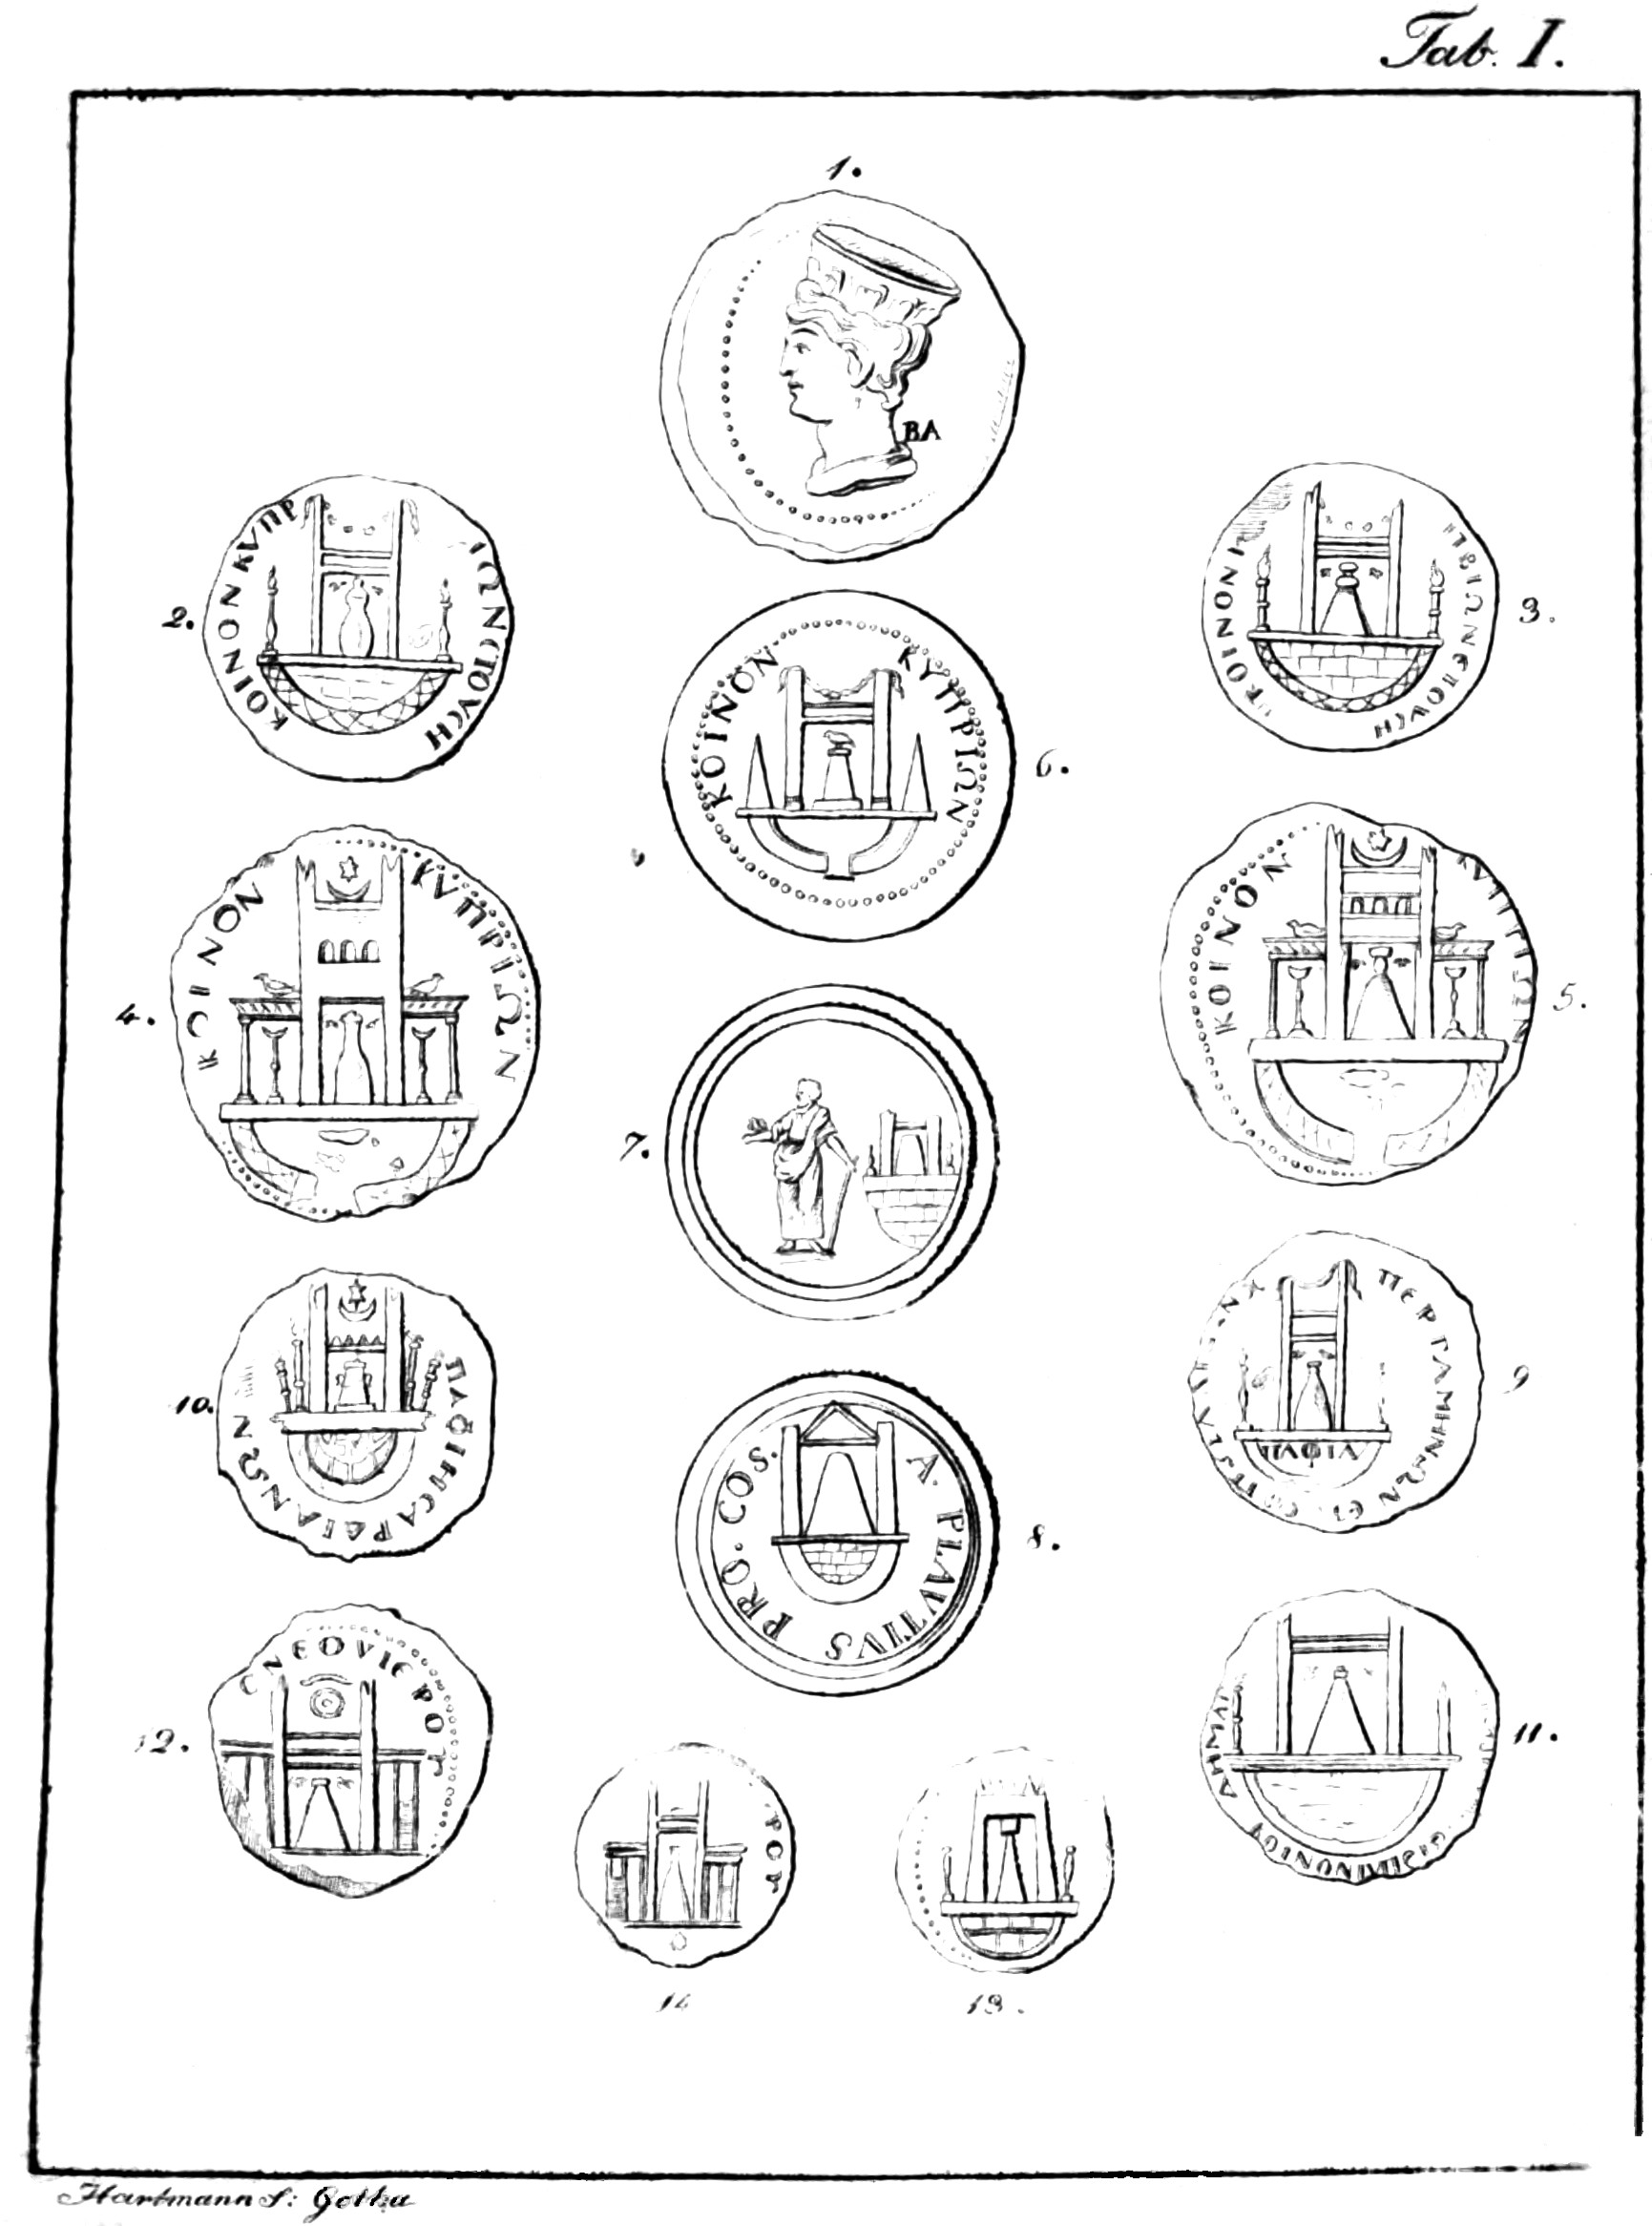
\includegraphics[width=0.95\textwidth,keepaspectratio]{tab1.jpg}
\end{figure}
\vspace*{\fill}
\clearpage
\vspace*{\fill}
\begin{figure}[H]
\centering
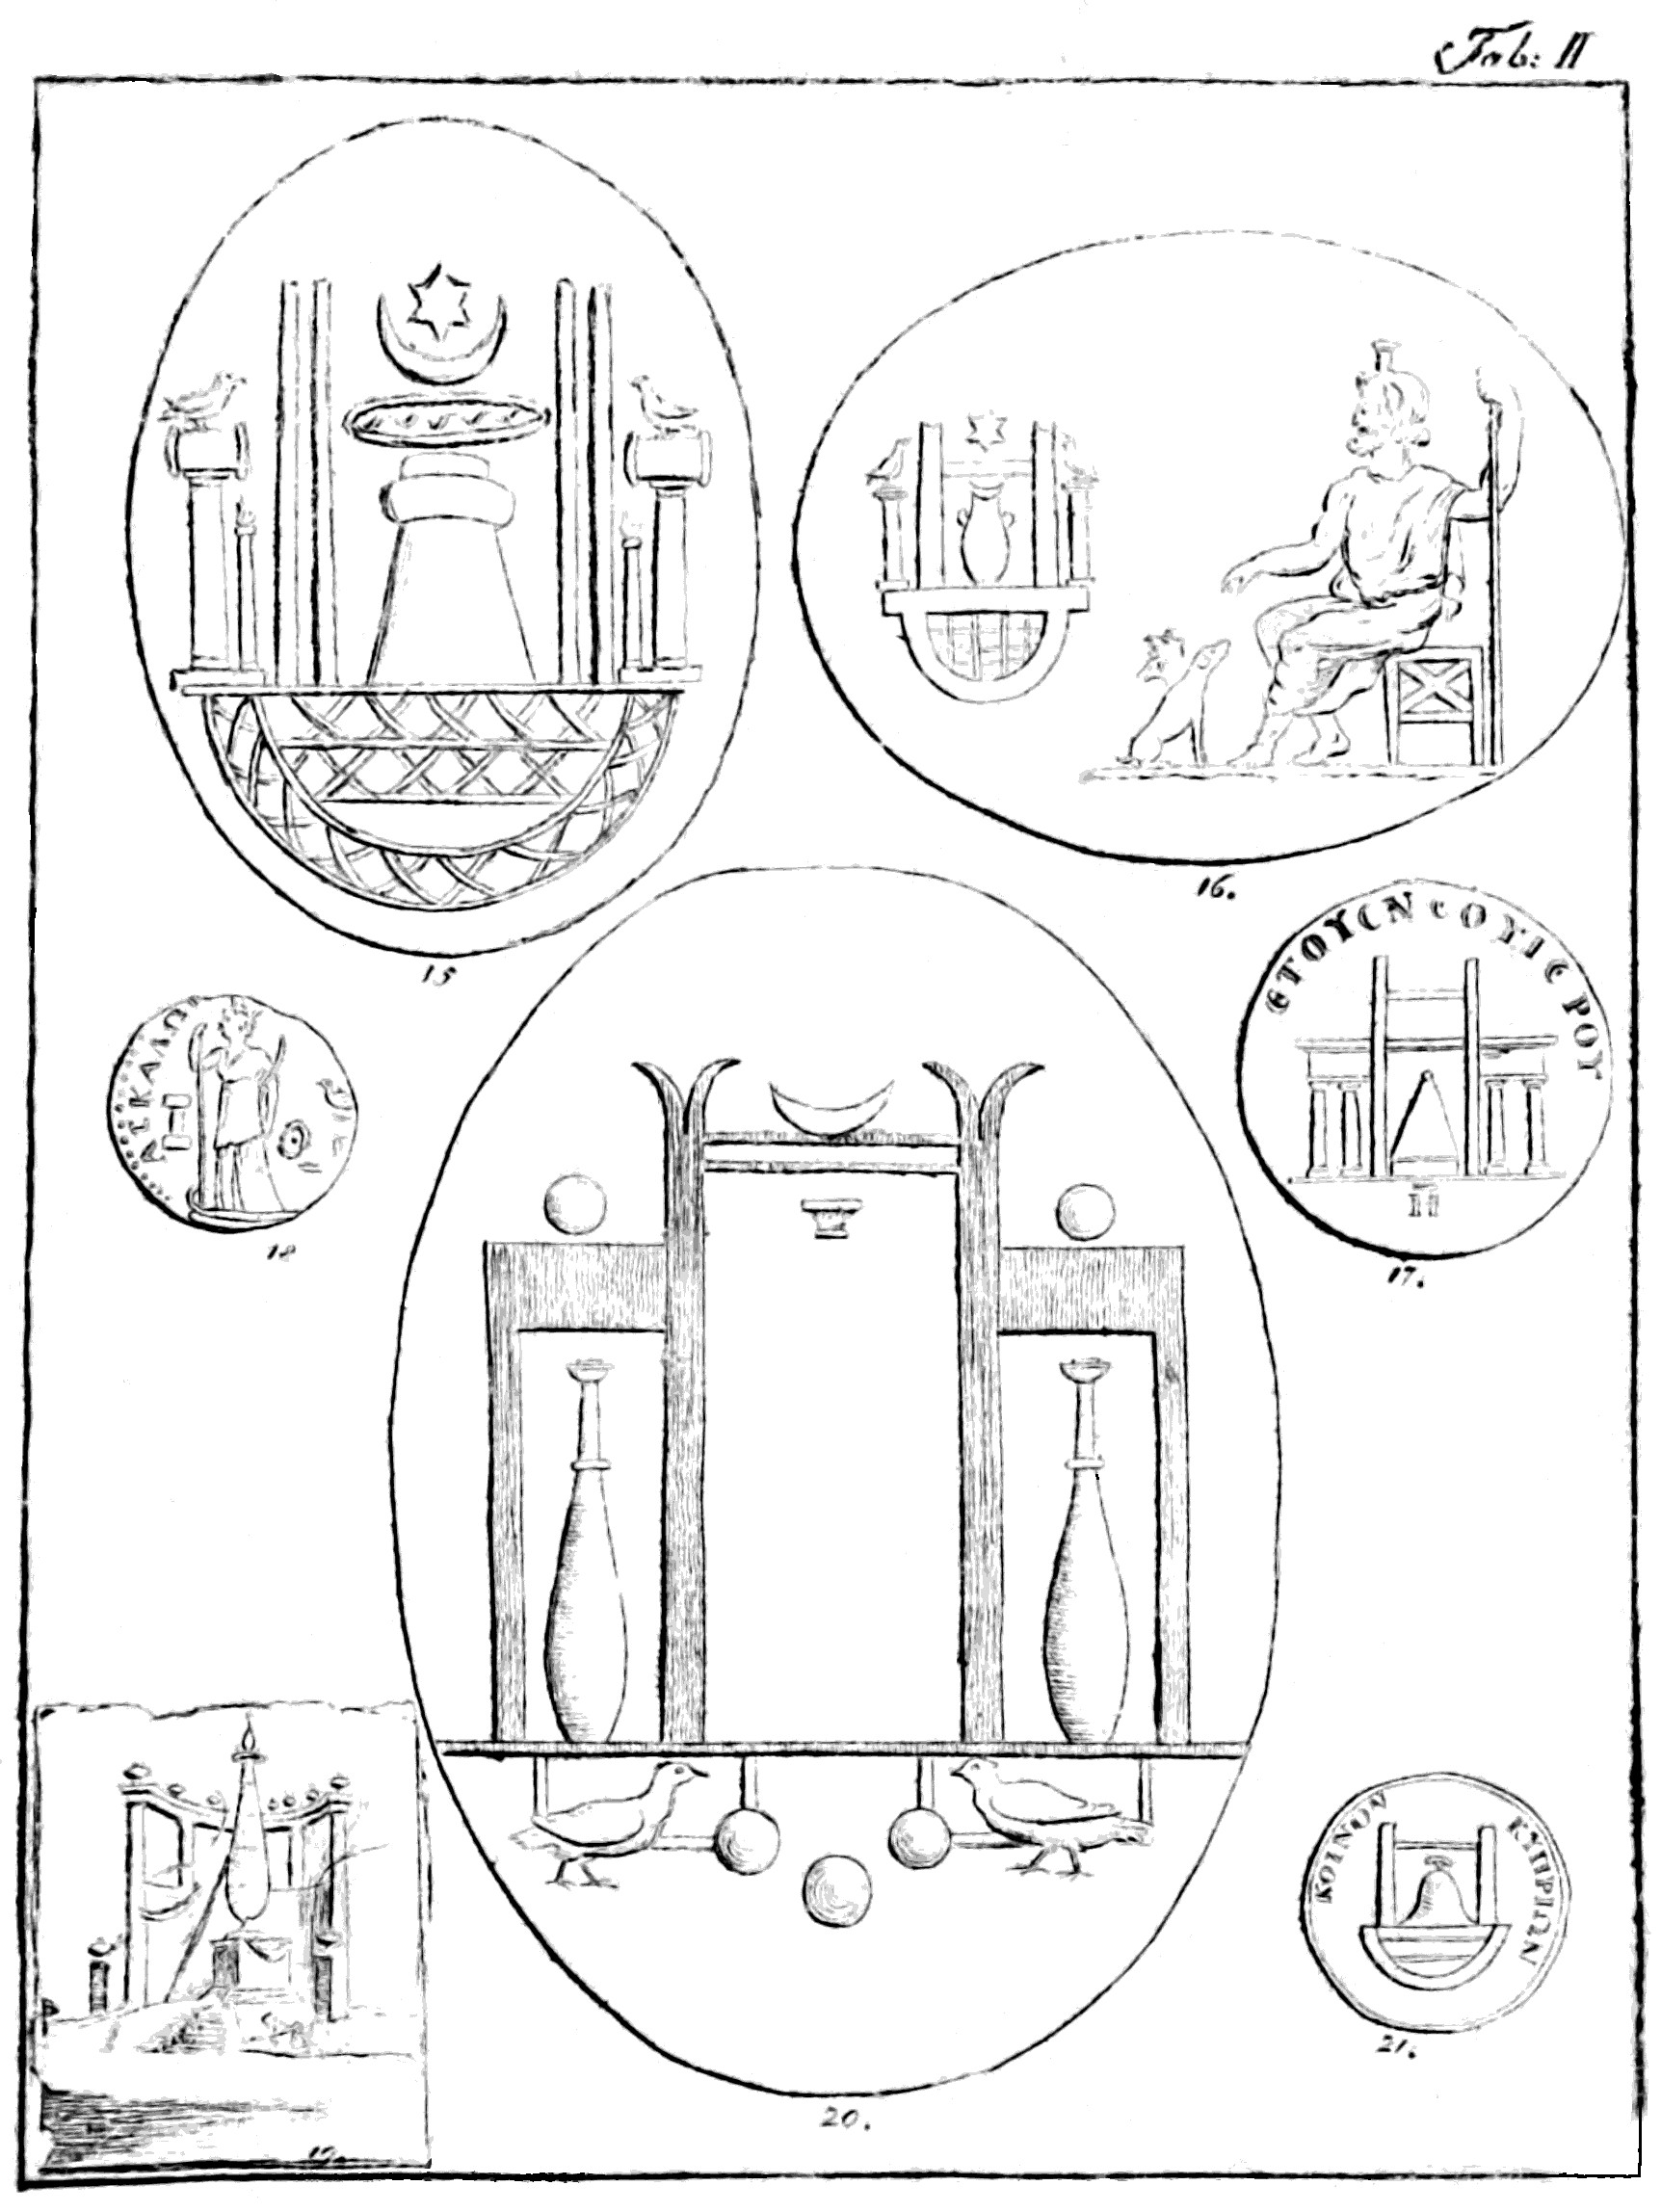
\includegraphics[width=0.95\textwidth,keepaspectratio]{tab2.jpg}
\end{figure}
\vspace*{\fill}
\clearpage
\begin{figure}[H]
\centering
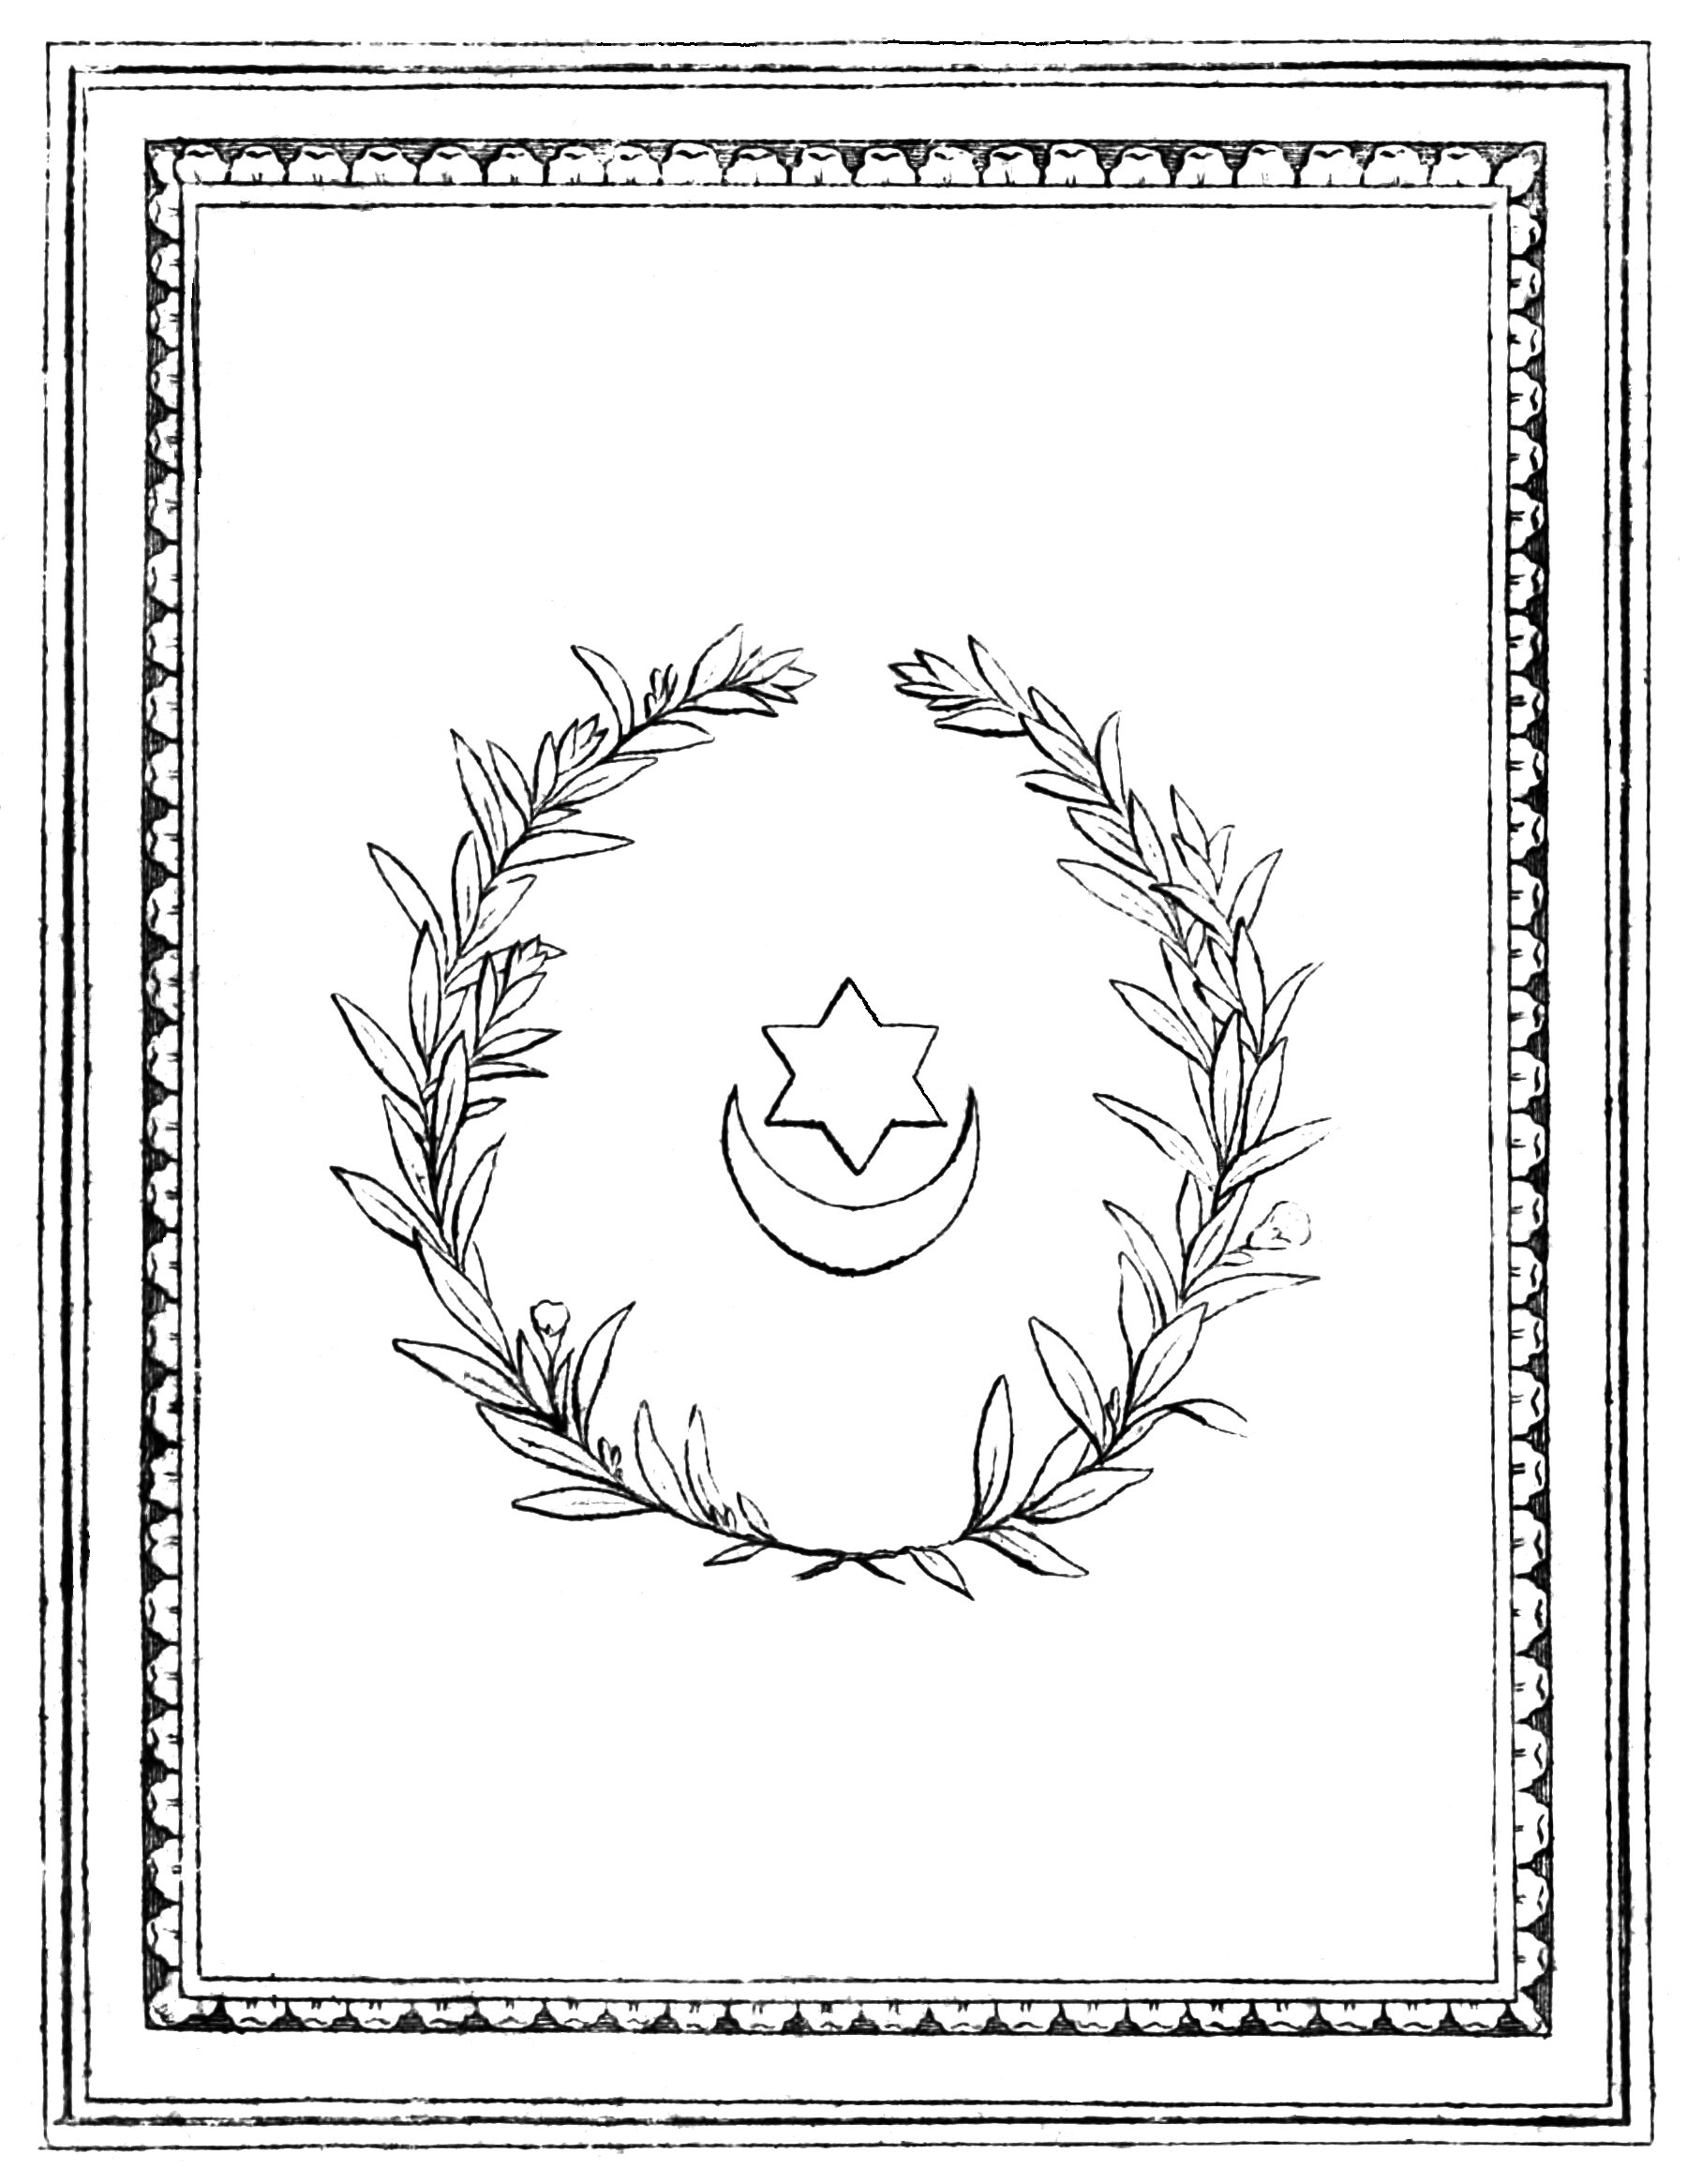
\includegraphics[width=0.95\textwidth,keepaspectratio]{fig2.jpg}
\end{figure}
\clearpage
\end{document}
